% !TeX document-id = {8fc77b15-3c07-42e1-8a11-7509577bf4d2}
% !TeX TXS-program:compile = txs:///xelatex/[--shell-escape]
% !TeX spellcheck = en_GB

%https://people.cs.georgetown.edu/jthaler/ProofsArgsAndZK.pdf


%\begin{frame}[allowframebreaks]{Table of Contents}
%\begin{itemize}
%\item Ethereum L1 Basics
%  \begin{itemize}
%  \item L1 execution layer
%  \item Data availability sharding scheme
%  \end{itemize}
%\item L2 Basics
%  \begin{itemize}
%  \item Optimistic execution
%  \item Succinct execution verification
%  \item Provers
%  \item \begin{Compression
%  \item Proto-danksharding
%  \end{itemize}
%
%\framebreak
%\item Proof generation
%  \begin{itemize}
%  \item Execution trace matrix
%  \item Witness and fixed columns
%  \item Executor: single computation or general purpose
%  \item zkASM 
%  \item Ethereum ROM and forkId
%  \item Constraints and PIL
%  \item Publics and privates
%  \item Generating and verifying proofs
%  \end{itemize}
%
%\framebreak
%\item Execution trace design
%  \begin{itemize}
%  \item Matrix shape
%  \item Secondary execution trace matrices
%  \item Lookup arguments
%  \item Delegated operation checks
%  \item Monolithic proofs
%  \end{itemize}
%
%\framebreak
%\item Basic zkEVM L2 processing
%  \begin{itemize}
%  \item Storage state machine
%  \item HashDB
%  \item First design of proof publics (inputs and outputs)
%  \item Consolidated state
%  \item Throughput limitations: prover-time and block-time
%  \item Sequencer and L2 transactions pool
%  \item Closing the batch and L2 transaction pre-execution.
%  \item L2 Ether supply.
%  \item Accumulated Input Hash
%  \item Virtual state
%  \item The “prove anything” paradigm
%  \item zkCounters
%  \item Variable degree composite proof (vadcop)
%  \item Prove anything and forced batches
%  \item Proof recursion and aggregation
%  \item Aggregator and its inputs/outputs
%  \item Trusted state
%  \item Node JSON RPC
%  \item L1 block, L2 block and L2 batch
%  \item Custom endpoints
%  \item Reorganizations and Sychronizer
%  \item StateDB
%  \end{itemize}
%
%\framebreak
%\item Bridge
%\item Forced Batches
%\item Fees and incentives
%  \begin{itemize}
%  \item chicken and egg with L2 Eth.
%We can start with L2 funds.
%There is another option (with a forced tx)
%  \end{itemize}
%\item Implementation
%  \begin{itemize}
%  \item Software components
%  \item Services
%  \item Detailed transaction flows
%  \item gRPCs
%  \item Trustless node
%  \end{itemize}
%
%\framebreak
%\item Module: zkEVM devops
%  \begin{itemize}
%  \item Staring an L1 node
%  \item Configuration files
%  \item Start the infrastructure
%  \item Logs (datadog, grafana, DBs, etc.)
%  \item Run the infrastructure
%  \item Hardware specs
%  \item Pool management
%  \item Slow executor: pending batches pool increase
%  \item Blocked addresses
%  \item L1 gas problems
%  \item Migrations, snapshots, restarting the node, etc.
%  \item Gas estimation
%  \end{itemize}
%
%\framebreak
%\item Module: Smart contracts
%  \begin{itemize}
%  \item Security mechanisms
%  \item Upgradability
%  \item Exit Merkle trees
%  \end{itemize}
%
%\framebreak
%\item Module: Prover and cryptography
%  \begin{itemize}
%  \item 
%  \end{itemize}
%\end{itemize}
%\end{frame}




\documentclass[10pt,english,handout,xcolor=table,aspectratio=169]{beamer} % Without animations (for printing)

%%%%%%%%%%%%%%%%%%%%%%%%%%%%%
% What I need to compile: `  %
%%%%%%%%%%%%%%%%%%%%%%%%%%%%%

% sudo apt install texlive-xelatex texlive-latex-extra texlive-generic-extra
% sudo apt install python-pip
% pip install pygments pygments-lexer-babylon pygments-lexer-solidity

% ---> IMPORTANT  <---
% This file should be compiled with XeTeX (http://xetex.sourceforge.net/)
% because using Unicode and modern font files is infinitely easier
% ---> IMPORTANT <---

%tlmgr manages an existing TeX Live installation, both packages and configuration options:
%sudo tlmgr update --self --all --reinstall-forcibly-removed

%%%%%%%%%%%%%%%%%%%%%%%%%%%%%%%%%%%%%%%%%%%%%%%%%%%%%%%%%%
% Note for ubuntu 16.04, minted from repo has a bug!!
% We use sty files from 18.04 (in ~/tmp/sty-18.04):

%sudo cp ~/tmp/sty-18.04/minted* /usr/share/texlive/texmf-dist/tex/latex/minted
%sudo mkdir /usr/share/texlive/texmf-dist/tex/latex/fvextra
%sudo cp ~/tmp/sty-18.04/fvextra.sty /usr/share/texlive/texmf-dist/tex/latex/fvextra
%sudo texhash
%%%%%%%%%%%%%%%%%%%%%%%%%%%%%%%%%%%%%%%%%%%%%%%%%%%%%%%%%%

%iosevka font (not used now)
%get: https://github.com/be5invis/Iosevka/releases/download/v2.0.0/02-iosevka-term-2.0.0.zip

%Fira font (currently used):
% https://github.com/mozilla/Fira/releases/tag/4.202
% wget https://github.com/mozilla/Fira/archive/4.202.zip
% unzip 4.202.zip
% cd Fira-4.202
% sudo mkdir -p /usr/share/fonts/opentype/fira
% sudo mkdir -p /usr/share/fonts/truetype/fira
% sudo find . -name "*.otf" -exec cp {} /usr/share/fonts/opentype/fira/ \;
% sudo find . -name "*.ttf" -exec cp {} /usr/share/fonts/truetype/fira/ \;
% sudo fc-cache -fv

%%%% Some useful latex:

%\begin{columns}
%\begin{column}{0.48\textwidth}
%\end{column}
%\begin{column}{0.48\textwidth}
%\end{column}
%\end{columns}

%\setbeamertemplate{itemize/enumerate body begin}{\small  }
%\setbeamertemplate{itemize/enumerate subbody begin}{\footnotesize }
%\setbeamertemplate{itemize/enumerate subsubbody begin}{\scriptsize }

%\begin{lstlisting}[style=termt]
%\end{lstlisting}

%\begin{frame}[fragile]\frametitle{}
%\begin{itemize}
%\item
%\end{itemize}
%\end{frame}


\usepackage{units}
\usepackage{csquotes}
%\usepackage[utf8]{inputenc}
%\usepackage[T1]{fontenc}
\usepackage{times}
\usepackage{textcomp}
\frenchspacing
\usepackage{booktabs}

%% New Metropolis
\usetheme[progressbar=frametitle,block=fill,numbering=fraction]{metropolis}
\setbeamerfont{footnote}{size=\tiny}
\setbeamercolor{background canvas}{bg=white}

\usepackage{fontspec}
\setmonofont{Iosevka Term}

% This package controls how hyperlinks are displayed
% https://es.overleaf.com/learn/latex/Hyperlinks
\usepackage{hyperref}
\hypersetup{colorlinks=true,linkcolor=,urlcolor={blue!80!black}}

%%\usepackage{xcolor}
%%\usetheme{Hannover}
%%\usecolortheme[RGB={51,92,133}]{structure}
%%\setbeamertemplate{navigation symbols}{}
%%\setbeamertemplate{blocks}[rounded][shadow=true] %blocks shape
%%%colors for blocks
%%\x{alertblue}{RGB}{51, 92, 133}
%%\xdefinecolor{alertbox}{RGB}{240, 240, 230}
%%\mode<presentation>{
%%%\usebackgroundtemplate{
%%%\hspace{7cm}\includegraphics[width=7cm]{\webdir/websockets/figures/upc.jpg}
%%%}
%%%Definitions of block colors
%%\setbeamercolor{block title}{fg=white,bg=alertblue}
%%\setbeamercolor{block title alerted}{fg=white, bg=red}
%%\setbeamercolor{block title example}{fg=white, bg=darkgray}
%%\setbeamercolor{block body}{bg=alertbox}
%%\setbeamercolor{block body alerted}{bg=alertbox}
%%\setbeamercolor{block body example}{bg=alertbox}
%%}
%%% \usepackage{svnkw}
%%% \usepackage{ifthen}
%%% \svnid{$Id: introduction.tex 11 2011-02-21 19:27:38Z juanjo $}
%%% \setbeamertemplate{footline}{\ifthenelse{\equal{\theframenumber}{1}}{Version:~ \svnfilerev ~~ \svnfiledate}{} \hfill
%%% \insertframenumber/\inserttotalframenumber}
%%\setbeamertemplate{footline}{\hfill \insertframenumber/\inserttotalframenumber}


\usepackage{dirtree}
\renewcommand*\DTstyle{\ttfamily\scriptsize}
%\renewcommand*\DTstyle{\ttfamily\textcolor{red}}

\usepackage{wasysym} % For checkboxes:  \CheckedBox \Square

%%%%%%%%%%%%%%%%%%%%%%%%%%%%%%%%%%%%%%%%
% BEGIN lstlistings                    %
%%%%%%%%%%%%%%%%%%%%%%%%%%%%%%%%%%%%%%%%

\usepackage{showexpl}% already includes listings package
% The listings package defines an internal command for replacements within filenames.
% One of these replacements replaces - with \textendash.
% You can redefine this command to make the hyphens actual hyphens:
\makeatletter
\def\lst@filenamerpl{_\textunderscore $\textdollar}
\makeatother
\lstset{frame=shadowbox, basicstyle=\footnotesize\ttfamily, showstringspaces=false,
rulesepcolor=\color{black}, upquote=true}
% \lstset{language=bash, frame=shadowbox, basicstyle=\footnotesize, showstringspaces=false,
% rulesepcolor=\color{black}, upquote=true, }
\lstdefinestyle{scriptStyle}{
    basicstyle=\footnotesize,% control font of code
    preset=\footnotesize,% adjust font size of output
    numbers=left, numberstyle=\tiny, stepnumber=1, numbersep=5pt,
    frame=tlbr,
    pos=r,% want output on rightbackgroundcolor=\color{yellow!30},
    width=0.50\linewidth,
}

\lstdefinestyle{terms}{
    basicstyle=\scriptsize\ttfamily,% control font of code
    preset=\footnotesize,% adjust font size of output
}

\lstdefinestyle{termt}{
    basicstyle=\tiny\ttfamily,% control font of code
    preset=\footnotesize,% adjust font size of output
}

\lstdefinestyle{verb}{
    basicstyle=\footnotesize,% control font of code
    preset=\footnotesize,% adjust font size of output
    frame=tlbr,
    pos=r,% want output on right
%     backgroundcolor=\color{yellow!30},
    width=0.50\linewidth,
}

\lstdefinestyle{verbs}{
    basicstyle=\scriptsize,% control font of code
    preset=\scriptsize,% adjust font size of output
    frame=tlbr,
    pos=r,% want output on right
%     backgroundcolor=\color{yellow!30},
    width=0.50\linewidth,
}

\lstdefinestyle{verbt}{
    basicstyle=\tiny\ttfamily,% control font of code
    preset=\tiny\ttfamily,% adjust font size of output
    frame=tlbr,
    pos=r,% want output on right
%     backgroundcolor=\color{yellow!30},
    width=0.50\linewidth,
}

%%%%%%%%%%%%%%%%%%%%%%%%%%%%%%%%%%%%%%%%
% END lstlistings                      %
%%%%%%%%%%%%%%%%%%%%%%%%%%%%%%%%%%%%%%%%

%%%%%%%%%%%%%%%%%%%%%%%%%%%%%%%%%%%%%%%%
% BEGIN Code Highlighting Environments %
%%%%%%%%%%%%%%%%%%%%%%%%%%%%%%%%%%%%%%%%

%sudo apt install texlive-latex-extra
%sudo apt install python-pip
%pip install pygments
%pip install pygments-lexer-babylon  #contains JSX
%pip install pygments-lexer-solidity

%pip install pygments pygments-lexer-babylon pygments-lexer-solidity



\usepackage{tcolorbox}
\tcbuselibrary{minted,skins,listings}
\definecolor{mybg}{rgb}{0.96,0.96,0.98}
\definecolor{nicegreen}{rgb}{0.55, 0.71, 0.0}

\newtcblisting{js}{
  listing engine=minted,
  colback=mybg,
  colframe=black!30,
  listing only,
  minted style=tango,
  minted language=js,
  minted options={linenos=true,texcl=true,fontsize=\tiny},
  left=0.2mm,
  top=0cm,
  bottom=0cm,
  boxrule=0.1mm
}


\newtcblisting{js-normalsize}{
  listing engine=minted,
  colback=mybg,
  colframe=black!30,
  listing only,
  minted style=tango,
  minted language=js,
  minted options={linenos=true,texcl=true,fontsize=\normalsize},
  left=0.2mm,
  top=0cm,
  bottom=0cm,
  boxrule=0.1mm
}



\newtcblisting{js-footnotesize}{
  listing engine=minted,
  colback=mybg,
  colframe=black!30,
  listing only,
  minted style=tango,
  minted language=js,
  minted options={linenos=true,texcl=true,fontsize=\footnotesize},
  left=0.2mm,
  top=0cm,
  bottom=0cm,
  boxrule=0.1mm
}



\newtcblisting{js-scriptsize}{
  listing engine=minted,
  colback=mybg,
  colframe=black!30,
  listing only,
  minted style=tango,
  minted language=js,
  minted options={linenos=true,texcl=true,fontsize=\scriptsize},
  left=0.2mm,
  top=0cm,
  bottom=0cm,
  boxrule=0.1mm
}


\newtcblisting{python}{
  listing engine=minted,
  colback=mybg,
  colframe=black!30,
  listing only,
  minted style=tango,
  minted language=python,
  minted options={linenos=true,texcl=true,fontsize=\tiny},
  left=0.2mm,
  top=0cm,
  bottom=0cm,
  boxrule=0.1mm
}


\newtcblisting{clang}{
  listing engine=minted,
  colback=mybg,
  colframe=black!30,
  listing only,
  minted style=tango,
  minted language=c,
  minted options={linenos=true,texcl=true,fontsize=\tiny},
  left=0.2mm,
  top=0cm,
  bottom=0cm,
  boxrule=0.1mm
}

\newtcblisting{php}{
  listing engine=minted,
  colback=mybg,
  colframe=black!30,
  listing only,
  minted style=tango,
  minted language=php,
  minted options={linenos=true,texcl=true,fontsize=\tiny},
  left=0.2mm,
  top=0cm,
  bottom=0cm,
  boxrule=0.1mm
}


\newtcblisting{mytext}{
  listing engine=minted,
  colback=mybg,
  colframe=black!30,
  listing only,
  minted style=bw,
  minted language=text,
  minted options={linenos=true,texcl=true,fontsize=\tiny},
  left=0.2mm,
  top=0cm,
  bottom=0cm,
  boxrule=0.1mm
}

\newtcblisting{htmlng2}{
  listing engine=minted,
  colback=mybg,
  colframe=black!30,
  listing only,
  minted style=tango,
  minted language=html+ng2,
  minted options={linenos=true,texcl=true,fontsize=\tiny},
  left=0.2mm,
  top=0cm,
  bottom=0cm,
  boxrule=0.1mm
}


\newtcblisting{http}{
  listing engine=minted,
  colback=mybg,
  colframe=black!30,
  listing only,
  minted style=tango,
  minted language=http,
  minted options={linenos=true,texcl=true,fontsize=\tiny},
  left=0.2mm,
  top=0cm,
  bottom=0cm,
  boxrule=0.1mm
}



\newtcblisting{jsx}{
  listing engine=minted,
  colback=mybg,
  colframe=black!30,
  listing only,
  minted style=tango,
  minted language=jsx,
  minted options={linenos=true,texcl=true,fontsize=\tiny},
  left=0.2mm,
  top=0cm,
  bottom=0cm,
  boxrule=0.1mm
}



\newtcblisting{ts}{
  listing engine=minted,
  colback=mybg,
  colframe=black!30,
  listing only,
  minted style=tango,
  minted language=ts,
  minted options={linenos=true,texcl=true,fontsize=\tiny},
  left=0.2mm,
  top=0cm,
  bottom=0cm,
  boxrule=0.1mm
}


\newtcblisting{bash}{
  listing engine=minted,
  colback=mybg,
  listing only,
  minted style=tango,
  minted language=bash,
  minted options={linenos=true,texcl=true,fontsize=\tiny},
  left=0.2mm,
  top=0cm,
  bottom=0cm,
  colframe=black!30,
  boxrule=0.1mm
}

\newtcblisting{json}{
  listing engine=minted,
  colback=mybg,
  colframe=black!30,
  listing only,
  minted style=tango,
  minted language=json,
  minted options={linenos=true,texcl=true,fontsize=\tiny},
  left=0.2mm,
  top=0cm,
  bottom=0cm,
  boxrule=0.1mm
}

\newtcblisting{xml}{
  listing engine=minted,
  colback=mybg,
  colframe=black!30,
  listing only,
  minted style=tango,
  minted language=xml,
  minted options={linenos=true,texcl=true,fontsize=\tiny},
  left=0.2mm,
  top=0cm,
  bottom=0cm,
  boxrule=0.1mm
}

\newtcblisting{yaml}{
  listing engine=minted,
  colback=mybg,
  colframe=black!70,
  listing only,
  minted style=tango,
  minted language=yaml,
  minted options={linenos=true,texcl=true,fontsize=\tiny},
  left=0.2mm,
  top=0cm,
  bottom=0cm,
  boxrule=0.1mm
}


\newtcblisting{html}{
  listing engine=minted,
  colback=mybg,
  colframe=black!70,
  listing only,
  minted style=tango,
  minted language=html,
  minted options={linenos=true,texcl=true,fontsize=\tiny},
  left=0.2mm,
  top=0cm,
  bottom=0cm,
  boxrule=0.1mm
}


\newtcblisting{css}{
  listing engine=minted,
  colback=mybg,
  colframe=black!70,
  listing only,
  minted style=tango,
  minted language=css,
  minted options={linenos=true,texcl=true,fontsize=\tiny},
  left=0.2mm,
  top=0cm,
  bottom=0cm,
  boxrule=0.1mm
}

\newtcblisting{solidity}{
  listing engine=minted,
  colback=mybg,
  colframe=black!70,
  listing only,
  minted style=tango,
  minted language=solidity,
  minted options={linenos=true,texcl=true,fontsize=\tiny},
  left=0.2mm,
  top=0cm,
  bottom=0cm,
  boxrule=0.1mm
}


\newtcblisting{graphql}{
  listing engine=minted,
  colback=mybg,
  colframe=black!70,
  listing only,
  minted style=tango,
  minted language=js,
  minted options={linenos=true,texcl=true,fontsize=\tiny},
  left=0.2mm,
  top=0cm,
  bottom=0cm,
  boxrule=0.1mm
}


% grpc and protobuf from google
\newtcblisting{proto}{
  listing engine=minted,
  colback=mybg,
  colframe=black!70,
  listing only,
  minted style=tango,
  minted language=proto,
  minted options={linenos=true,texcl=true,fontsize=\tiny},
  left=0.2mm,
  top=0cm,
  bottom=0cm,
  boxrule=0.1mm
}


\lstdefinelanguage{circom}{
	keywords=[1]{signal, input, output, <==, ==>, ===}, % generic keywords including crypto operations
  keywordstyle=[1]\color{blue!70!}\bfseries,
	keywords=[3]{pragma, include},
  keywordstyle=[3]\color{brown}\bfseries,
	keywords=[4]{for, if, var, else},
	keywordstyle=[4]\color{teal}\bfseries,
	keywords=[5]{template, component},
	keywordstyle=[5]\color{violet}\bfseries,
	identifierstyle=\color{black},
	sensitive=false,
	comment=[l]{//},
	morecomment=[s]{/*}{*/},
	commentstyle=\color{green!40!black}\ttfamily,
	stringstyle=\color{blue}\ttfamily,
%	morestring=[b]',
%	morestring=[b]"
}

\newtcblisting{circom}{
  listing engine=listings,
  colback=mybg,
  colframe=black!70,
  listing only,
  listing options={
    language={circom},
	basicstyle=\tiny\ttfamily,
    frame=none,
	numbers=left,
	numberstyle=\tiny,
	numbersep=9pt,
	tabsize=2,
	breaklines=true,
	showtabs=false,
	captionpos=b
  },
  left=0.2mm,
  top=0cm,
  bottom=0cm,
  boxrule=0.1mm
}



\lstdefinelanguage{Pil}{
	keywords=[1]{pol, commit, constant, in, is, connect, public, namespace}, % generic keywords including crypto operations
  keywordstyle=[1]\color{blue!70!}\bfseries,
	keywords=[3]{include}, % modules
  keywordstyle=[3]\color{brown}\bfseries,
	keywords=[4]{},% types; money and time units
	keywordstyle=[4]\color{teal}\bfseries,
	keywords=[5]{field, bool, u32, u16, u8},	% environment variables
	keywordstyle=[5]\color{violet}\bfseries,
	identifierstyle=\color{black},
	sensitive=false,
	comment=[l]{//},
	morecomment=[s]{/*}{*/},
	commentstyle=\color{green!40!black}\ttfamily,
	stringstyle=\color{blue}\ttfamily,
%	morestring=[b]',
%	morestring=[b]"
}

\newtcblisting{pil}{
  listing engine=listings,
  colback=mybg,
  colframe=black!70,
  listing only,
  listing options={
    language={Pil},
	basicstyle=\tiny\ttfamily,
    frame=none,
	numbers=left,
	numberstyle=\tiny,
	numbersep=9pt,
	tabsize=2,
	breaklines=true,
	showtabs=false,
	captionpos=b
  },
  left=0.2mm,
  top=0cm,
  bottom=0cm,
  boxrule=0.1mm
}


\lstdefinelanguage{zkASM}{
    keywords=[1]{VAR, GLOBAL, CONST, CONSTL, INCLUDE},
    keywordstyle=[1]\color{blue!70!}\bfseries,
    keywords=[3]{},
    keywordstyle=[3]\color{brown}\bfseries,
    keywords=[4]{A, B, C, D, E, SR, CTX, SP, PC, GAS, zkPC, RR, STEP, MAXMEM, HASHPOS, RCX, ROTL_C, CNT_ARITH, CNT_BINARY, CNT_KECCAK_F, CNT_MEM_ALIGN, CNT_PADDING_PG, CNT_POSEIDON_G},
    keywordstyle=[4]\color{teal}\bfseries,
    keywords=[5]{MSTORE, MLOAD, MEM_ALIGN_RD, MEM_ALIGN_WR, MEM_ALIGN_WR8, ASSERT, HASHK, HASHKLEN, HASHKDIGEST, HASHP, HASHPLEN, HASHPDIGEST, HASHP1, HASHK1, SLOAD, STORE, ARITH, ARITH_ECADD_DIFFERENT, ARITH_ECADD_SAME, LT, SLT, EQ, AND, OR, XOR, ADD, SUB, INST_MAP_ROM, SYS, MEM, STACK, JMP, JMPN, JMPC, JMPZ, JMPNZ, JMPNC, REPEAT, CALL, RETURN},
    keywordstyle=[5]\color{violet}\bfseries,
    identifierstyle=\color{black},
    sensitive=false,
    comment=[l]{;},
    commentstyle=\color{green!40!black}\ttfamily,
    stringstyle=\color{blue}\ttfamily,
    %	morestring=[b]',
    %	morestring=[b]"
}



\newtcblisting{zkasm}{
    listing engine=listings,
    colback=mybg,
    colframe=black!70,
    listing only,
    listing options={
        language={zkASM},
        basicstyle=\tiny\ttfamily,
        frame=none,
        numbers=left,
        numberstyle=\tiny,
        numbersep=9pt,
        tabsize=2,
        breaklines=true,
        showtabs=false,
        captionpos=b
    },
    left=0.2mm,
    top=0cm,
    bottom=0cm,
    boxrule=0.1mm
}


%%%%%%%%%%%%%%%%%%%%%%%%%%%%%%%%%%%%%%%%
% END   Code Highlighting Environments %
%%%%%%%%%%%%%%%%%%%%%%%%%%%%%%%%%%%%%%%%


% Tikz Library
% https://www.iacr.org/authors/tikz/
\usepackage{tikz}
\usetikzlibrary{shapes,shapes.callouts,calc, arrows, positioning, matrix, intersections, decorations.markings}
\tikzset{point/.style={draw,fill,circle,inner sep=1pt}}
\tikzset{vertex/.style = {shape=circle,draw,minimum size=1.5em}}
\tikzset{edge/.style = {-}}
\tikzset{arrow/.style = {->}}


\newcommand{\mysquare}[1]{\tikz{\node[draw=#1,fill=#1,rectangle,minimum
width=0.2cm,minimum height=0.2cm,inner sep=0pt] at (0,0) {};}}

\newcommand{\mycircle}[1]{\tikz{\node[draw=#1,fill=#1,circle,minimum
width=0.2cm,minimum height=0.2cm,inner sep=0pt] at (0,0) {};}}

\newcommand{\mytriangle}[1]{\tikz{\node[draw=#1,fill=#1,isosceles
triangle,isosceles triangle stretches,shape border rotate=90,minimum
width=0.2cm,minimum height=0.2cm,inner sep=0pt] at (0,0) {};}}

\newcommand{\mystar}[1]{\tikz{\node[draw=#1,fill=#1,star,star points=5, star point ratio=2.25, minimum
width=0.2cm,minimum height=0.2cm,inner sep=0pt] at (0,0) {};}}


\newcommand{\plotcurve}[4][thick, every plot/.style={smooth}]{
  % plot curve y^2 = x^3 + a x + b in range [-#4,#4]^2
  % parameter 1 (optional): style options for curve (color, etc)
  % parameter 2: curve parameter a
  % parameter 3: curve parameter b
  % parameter 4: range to print
  % \draw[gray] (-3,-3) rectangle (3,3);
  \draw[->,>=latex,gray] (-#4,0) -- (#4,0);
  \draw[->,>=latex,gray] (0,-#4) -- (0,#4);
  \draw[name path=curve, #1] plot[id=curve#2#3, raw gnuplot] function {
    f(x,y) = y**2 - x**3 - #2*x - #3;
    set xrange [-#4:#4];
    set yrange [-#4:#4];
    set view 0,0;
    set isosample 50,50;
    set contour base;
    set cntrparam levels incre 0,0.1,0;
    unset surface;
    splot f(x,y);
  };
}

% For an explanation of the tangent coordinate system, check http://tex.stackexchange.com/a/25940
\tikzset{
  tangent/.style={
    decoration={markings, mark=at position #1 with {
      \coordinate (tangent point-\pgfkeysvalueof{/pgf/decoration/mark info/sequence number}) at (0pt,0pt);
      \coordinate (tangent unit vector-\pgfkeysvalueof{/pgf/decoration/mark info/sequence number}) at (1,0pt);
      \coordinate (tangent orthogonal unit vector-\pgfkeysvalueof{/pgf/decoration/mark info/sequence number}) at (0pt,1);
    }},
    postaction=decorate
  },
  use tangent/.style={
    shift=(tangent point-#1),
    x=(tangent unit vector-#1),
    y=(tangent orthogonal unit vector-#1)
  },
  use tangent/.default=1
}

% Alternative to tikz
\usepackage{pgfplots}
\pgfplotsset{compat=newest}

\usepackage{xspace}

% Bold Math
\renewcommand{\vec}[1]{\ensuremath{\boldsymbol{#1}}\xspace}
\newcommand{\vel}[3]{\ensuremath{\vec{#1_{#2}}(#3)}\xspace}


% Caligraphic Combiantions
\DeclareMathAlphabet{\mathpgoth}{OT1}{pgoth}{m}{n}
\newcommand{\plonk}{\ensuremath{\mathcal{P}\mathfrak{lon}\mathcal{K}}\xspace}
\newcommand{\fflonk}{\ensuremath{\mathcal{FF}\mathfrak{lon}\mathcal{K}}\xspace}
\newcommand{\plookup}{\ensuremath{\mathpgoth{plookup}}\xspace}



% Mathcal
\renewcommand{\P}{\mathcal{P}}
\renewcommand{\S}{\ensuremath{\mathcal{S}}\xspace}
\newcommand{\V}{\mathcal{V}}
% \renewcommand{\C}{\mathcal{C}}
\newcommand{\C}{\mathcal{C}}
\renewcommand{\H}{\mathcal{H}}


\newcommand{\FF}{\ensuremath{\mathbb{F}}\xspace}
\newcommand{\ZZ}{\ensuremath{\mathbb{Z}}\xspace}
\newcommand{\GG}{\ensuremath{\mathbb{G}}\xspace}

% PIL
\newcommand{\row}{\ensuremath{\mathtt{row}}\xspace}
\newcommand{\freeIn}{\ensuremath{\mathtt{freeIn}}\xspace}
\newcommand{\out}{\ensuremath{\mathtt{out}}\xspace}
\newcommand{\RESET}{\ensuremath{\mathtt{RESET}}\xspace}
\newcommand{\nextStep}{\ensuremath{\mathtt{'}}\xspace}
\newcommand{\carry}{\ensuremath{\mathtt{carry}}\xspace}
\newcommand{\att}{\ensuremath{\mathtt{a}}\xspace}
\newcommand{\btt}{\ensuremath{\mathtt{b}}\xspace}
\newcommand{\ctt}{\ensuremath{\mathtt{c}}\xspace}
\newcommand{\dtt}{\ensuremath{\mathtt{d}}\xspace}
\newcommand{\ett}{\ensuremath{\mathtt{e}}\xspace}
\newcommand{\ftt}{\ensuremath{\mathtt{f}}\xspace}
\newcommand{\SEL}{\ensuremath{\mathtt{SEL}}\xspace}
\newcommand{\sel}{\ensuremath{\mathtt{sel}}\xspace}
\newcommand{\add}{\ensuremath{\mathtt{add}}\xspace}
\newcommand{\ISLAST}{\ensuremath{\mathtt{ISLAST}}\xspace}

\newcommand{\QL}{\ensuremath{\mathtt{QL}}\xspace}
\newcommand{\QR}{\ensuremath{\mathtt{QR}}\xspace}
\newcommand{\QM}{\ensuremath{\mathtt{QM}}\xspace}
\newcommand{\QO}{\ensuremath{\mathtt{QO}}\xspace}
\newcommand{\QC}{\ensuremath{\mathtt{QC}}\xspace}

\newcommand{\SA}{\ensuremath{\mathtt{SA}}\xspace}
\newcommand{\SB}{\ensuremath{\mathtt{SB}}\xspace}
\newcommand{\SC}{\ensuremath{\mathtt{SC}}\xspace}

% Programs
\newcommand{\Multiplier}{\ensuremath{\mathsf{Multiplier}}\xspace}
\newcommand{\pilcom}{\ensuremath{\mathsf{pilcom}}\xspace}
\newcommand{\pilstark}{\ensuremath{\mathsf{pil-stark}}\xspace}

\usepackage{wasysym} % For checkboxes:  \CheckedBox \Square
%Use:
%\hfill \CheckedBox
%\hfill \Square


\AtBeginSection[]
{
   \begin{frame}
       \frametitle{Outline}
       \fontsize{9}{6}\selectfont % first is the fontsize, second separation
       \tableofcontents[currentsection]
   \end{frame}
}


\AtBeginSubsection[]
{
   \begin{frame}
       \setcounter{tocdepth}{2} %show only up to subsubsection
       \frametitle{Outline}
      \fontsize{10}{18}\selectfont 
       \tableofcontents[currentsubsection]
   \end{frame}
}


%\newcommand{\cbox}[2]{
%  \begin{center}
%  \begin{boxedminipage}{#1} #2 \end{boxedminipage}
%  \end{center}
%}

% Web for icons: https://www.flaticon.com/

%%%%%%%%%%%%%%%%%%%%%%%%%%
% To include GIT commits %
%%%%%%%%%%%%%%%%%%%%%%%%%%
% Two required libraries
%\usepackage{xstring}
%\usepackage{catchfile}
%\newcommand{\gitfolder}{../../../.git}             % Relative path to .git folder from .tex file
%\newcommand{\reponame}{worldbank/d4di}    % Name of account and repo. Will be included in URL
%\CatchFileDef{\headfull}{\gitfolder/HEAD}{}              % Get path to head file for checked out branch
%\StrGobbleRight{\headfull}{1}[\head]                      % Remove end of line character
%\StrBehind[2]{\head}{/}[\branch]                          % Parse out the path only
%\CatchFileDef{\commit}{\gitfolder/refs/heads/\branch}{}  % Get the content of the branch head
%\StrGobbleRight{\commit}{1}[\commithash]                  % Remove end of line character
% Build the URL to this commit based on the information we now have
%\newcommand{\commiturl}{\url{https://github.com/\reponame/commit/\commithash}}
%%%%%%%%%%%%%%%%%%%%%%%%%%
% END GIT commits        %
%%%%%%%%%%%%%%%%%%%%%%%%%%


\title{Demystifying a zkEVM}
\author{Web3FC 2024 \\
\\
\scriptsize
Ignasi Ramos <ignasi@polygon.technology>\\
Jose Luis Muñoz-Tapia <jose.luis.munoz@upc.edu> \\
\\
%Version: \commithash % Commit of our internal repo
}
\date{}



% Definitions of includes with if
\newif\ifPROF
\newif\ifEXTRA
\newif\ifEXTRAEXTRA

\newif\ifZEROSEC
\newif\ifSEC
\newif\ifSUBSEC
\newif\ifSUBSUBSEC
\newif\ifARCHMAP \ARCHMAPtrue
\newif\ifPILFOURBYTEEXAMPLE %\PILFOURBYTEEXAMPLEtrue
\newif\ifRPCQUERIES %\RPCQUERIEStrue


\newif\ifCOMMENT

%\EXTRAtrue
%\PROFtrue

% For setting the section's level
\newcommand{\mytitle}{title}
\SECtrue

% Columns with colors
\usepackage{colortbl}
\definecolor{Gray}{gray}{0.9}
\newcolumntype{a}{>{\columncolor{Gray}}c}

\newcommand{\definedir}[2]{\newcommand{#1}{#2}}
\definedir{\zkevmdir}{..}

\begin{document}
\begin{frame}
   \titlepage
\end{frame}
% !TeX document-id = {38ad272c-6b95-4178-b409-8ae7f3766667}
% !TeX spellcheck = en_US
% !TeX root = ../../build/architecture.tex
% !TeX TXS-program:compile = txs:///xelatex/[--shell-escape]


\renewcommand{\mytitle}{Ethereum Layer 1}
\ifZEROSEC \fi
\ifSEC \section{\mytitle{}}\fi
\ifSUBSEC \subsection{\mytitle{}}\fi
\ifSUBSUBSEC \subsubsection{\mytitle{}}\fi



\begin{frame}{Ethereum Layer 1}
\begin{figure}[H]
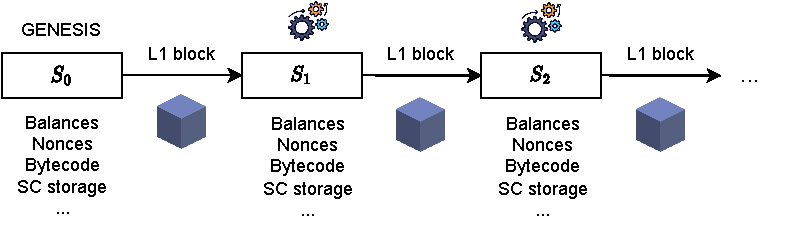
\includegraphics[width=0.8\columnwidth]{\zkevmdir/figures/concepts/layer1-ethereum/ethereum-layer1}
\end{figure}
\centering
Transactions in L1 blocks are \textbf{available} and \textbf{executed}.
\end{frame}




\begin{frame} {Representation of Each State}
  \begin{itemize}
    \item $S_i$ denotes a cryptographic summary of the data of state $i$.
    \item $S_i$ is implemented as the \textbf{root} of a Merkle Tree 
    that includes data items as leaves of the $i$-th state.
    \newline
    \begin{figure}[H]
      \centering
      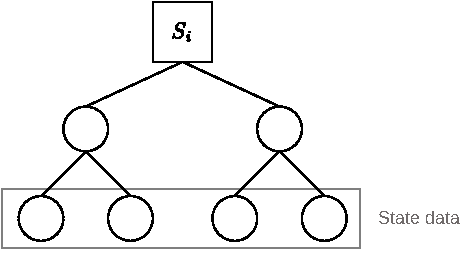
\includegraphics[width=0.4\columnwidth]{\zkevmdir/figures/concepts/layer1-ethereum/representation-state}
    \end{figure}
    % TODO Make figure smaller
  \end{itemize}
\end{frame}
% !TeX document-id = {38ad272c-6b95-4178-b409-8ae7f3766667}
% !TeX spellcheck = en_US
% !TeX root = ../../build/architecture.tex
% !TeX TXS-program:compile = txs:///xelatex/[--shell-escape]


\renewcommand{\mytitle}{The Road to Ethereum Scalability}
\ifZEROSEC \fi
\ifSEC \section{\mytitle{}}\fi
\ifSUBSEC \subsection{\mytitle{}}\fi
\ifSUBSUBSEC \subsubsection{\mytitle{}}\fi


\begin{frame} {Scaling Blockchain and the Scaling Trilemma}
\begin{block}{Scaling Blockchain}
When we talk about scaling blockchain, we talk about \textbf{increasing the number of processed transactions per second}.
\end{block}
\begin{itemize}
\item The term \textbf{scalability trilemma} was first coined by \textit{Vitalik Buterin} to describe the inherent tension between three properties that a high-performing blockchain platform must have:
  \begin{enumerate}
  \item Decentralization.
  \item Security.
  \item Scalability.
  \end{enumerate}
\item The trilemma refers to the belief that blockchain platforms can only achieve two of these three goals effectively.
\end{itemize}
\end{frame}



\begin{frame} {How to scale?}
  \textbf{Approach \#1}
  \begin{itemize}
    \item Increase transactions per block.
    \item This may lead many blockchain nodes to exhaust their resources.
    \item Therefore, this may trigger centralization (a network with only powerful nodes).
  \end{itemize}
  \textbf{Approach \#2}
  \begin{itemize}
    \item Do \textbf{sharding}, which means split the burden in shards.

    \item A node only deals with a \textit{portion} of the burden, i.e. with the operations
    in its shard.

    \item There are several approaches within the sharding strategy.
  \end{itemize}
\end{frame}






\begin{frame} {Approach \#2.a: Sharding for Data Availability and Execution}
  \begin{itemize}
    \item The first approach consists in using the current L1 chain as a \textit{consolidation chain}, 
    which will be renamed as the L1 \textbf{beacon chain}.
    \item Then, use \textbf{availability} and \textbf{execution} in each shard:

    \begin{figure}
      \centering
      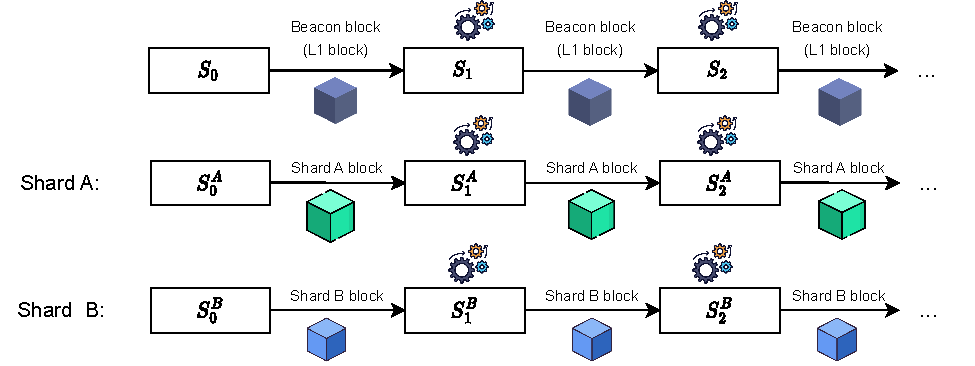
\includegraphics[width=0.9\columnwidth]{\zkevmdir/figures/concepts/road-to-scalability/execution-shard-chains.drawio}
    \end{figure}
  \end{itemize}
\end{frame}





\begin{frame} {Problems of Sharding with Data\_Availability+Execution}
The previous approach is a L1 design with \textbf{availability and execution} in each shard.

\vspace{0.15cm}
However, this produces a huge instability in Ethereum L1 specifications:
\begin{itemize}
\item L1 Ethereum is responsible for the managements of each of shard's states.
\item This includes the \textbf{execution} and \textbf{inter-shard messaging} when necessary.
\item This does not allow L1 \textbf{ossification}.
\end{itemize}
\end{frame}





\begin{frame}{Approach \#2.b: Data Availability Sharding and a Single Execution Layer}
\begin{itemize}
\item In this approach Ethereum specifications provide:
  \begin{enumerate}
  \item Just \textbf{ONE L1 execution layer} giving execution and availability (that is, the current L1).
  \item Data availability sharding scheme (\href{https://ethereum.org/ca/roadmap/danksharding}{danksharding}).
  \end{enumerate}
\begin{figure}
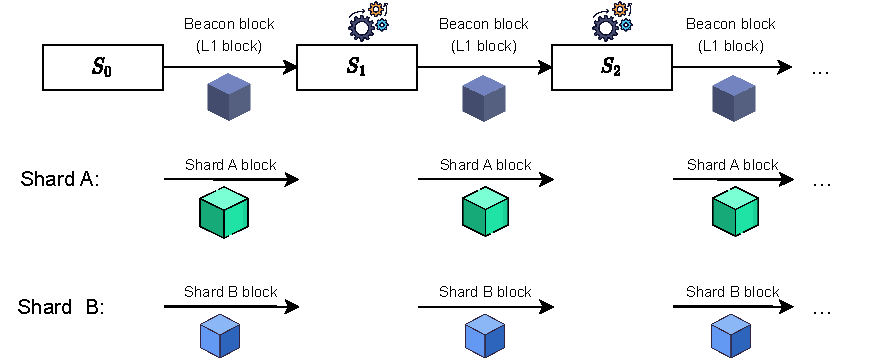
\includegraphics[width=0.8\columnwidth]{\zkevmdir/figures/concepts/road-to-scalability/data-shard-chains.drawio}
\end{figure}
\end{itemize}
\end{frame}




\begin{frame}{\texttt{blobs}}
\begin{columns}
\begin{column}{0.4\textwidth}
Instead of transactions, shard blocks contain \textbf{blobs} (binary large objects) that designed to be interpreted by a top layer.
\end{column}
\begin{column}{0.58\textwidth}
\begin{figure}
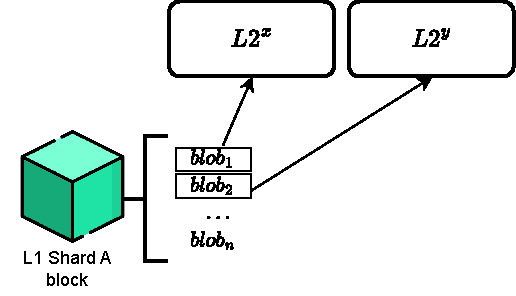
\includegraphics[width=0.8\columnwidth]{\zkevmdir/figures/concepts/road-to-scalability/block-of-blobs.drawio}
\end{figure}
\end{column}
\end{columns}
\end{frame}




\begin{frame}{L2 Layers}
\begin{itemize}
\item New top layers, called \textbf{L2 layers}, can be created on top of this L1 machinery.
\item L2's define how they manage the state: 
  \begin{itemize}
  \item A payment system with simple transactions.
  \item A token transfer system.
  \item A system with smart contracts.
  \end{itemize}
\item L2's also define how they use L1:
  \begin{itemize}
  \item The L1 execution layer.
  \item The data shards (when available\footnote{Regarding the current situation of data sharding,
  L1 data shards specification is still under develop (the \textbf{EIP 4484} is currently on the "review stage"). 
  For this reason, currently, all the scaling solutions use the availability of the execution layer.}).
  \end{itemize}
\end{itemize}
\end{frame}





\begin{frame}{Building a Layer 2}
\begin{columns}
\begin{column}{0.35\textwidth}
\begin{itemize}
\item Let's assume that our layer 2 is called x ($L2_x$).
\item The state of the layer x progresses with its L2 transactions.
\end{itemize}
\end{column}
\begin{column}{0.65\textwidth}
\begin{figure}
\includegraphics[width=\columnwidth]{\zkevmdir/figures/concepts/road-to-scalability/l2-state.drawio}
\end{figure}
\end{column}
\end{columns}

\begin{itemize}
\item There are many questions to answer to build an L2:
  \begin{enumerate}[a)]
  \item How users send L2 transactions and who receives them?
  \item How these L2 transactions are made publicly available (if so)?
  \item Who processes the L2 transactions and how, and, when 
  it is publicly considered that a new state is correctly computed?
  \item What type of applications the L2 supports? simple or rich processing?
  \end{enumerate}
\end{itemize}
\end{frame}
% !TeX document-id = {38ad272c-6b95-4178-b409-8ae7f3766667}
% !TeX spellcheck = en_US
% !TeX root = ../../build/architecture.tex
% !TeX TXS-program:compile = txs:///xelatex/[--shell-escape]


\renewcommand{\mytitle}{Layer 2 Scalability Strategies}
\ifZEROSEC \fi
\ifSEC \section{\mytitle{}}\fi
\ifSUBSEC \subsection{\mytitle{}}\fi
\ifSUBSUBSEC \subsubsection{\mytitle{}}\fi


\begin{frame}{Building a Layer 2}
\begin{columns}
\begin{column}{0.35\textwidth}
\begin{itemize}
\item Let's assume that our layer 2 is called x ($L2_x$).
\item The state of the layer x progresses with its L2 transactions.
\end{itemize}
\end{column}
\begin{column}{0.65\textwidth}
\begin{figure}
\includegraphics[width=\columnwidth]{\zkevmdir/figures/concepts/l2-scaling-strategies/l2-state.drawio}
\end{figure}
\end{column}
\end{columns}

\begin{itemize}
\item There are many questions to answer to build an L2:
  \begin{enumerate}[a)]
  \item How users send L2 transactions and who receives them?
  \item How these L2 transactions are made publicly available (if so)?
  \item Who processes the L2 transactions and how, and, when 
  it is publicly considered that a new state is correctly computed?
  \item What type of applications the L2 supports? simple or rich processing?
  \end{enumerate}
\end{itemize}
\end{frame}




\begin{frame}{Layer 2 Design: Sending L2 Transactions}
\textbf{Q.} How users send L2 transactions and who receives them?
  \begin{itemize}
  \item \textbf{Unicast}: an unicast communication with some (centralized) entity.
  \item \textbf{Peer-to-peer}: a peer-to-peer network where everybody (decentralized) receives the L2 transactions.
  \item \textbf{Smart contract}: a smart contract in the L1 execution layer (decentralized).
  \end{itemize}

\vspace{1em}

\begin{columns}[t]

\begin{column}{0.3 \textwidth}
\centering
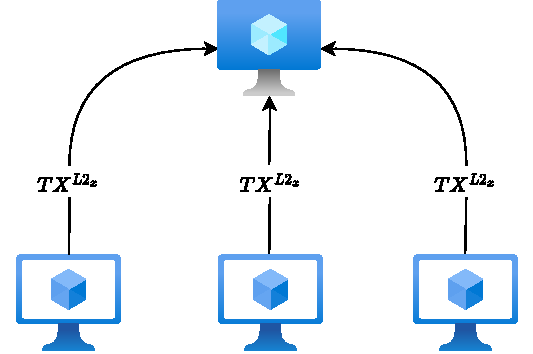
\includegraphics[width=.8\columnwidth]{\zkevmdir/figures/concepts/l2-scaling-strategies/unicast.drawio}
\textbf{Unicast}
\end{column}

\begin{column}{0.3 \textwidth}
\centering
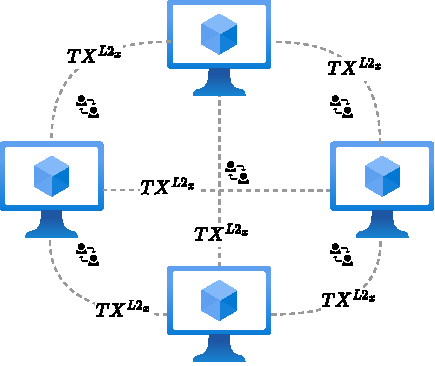
\includegraphics[width=.8\columnwidth]{\zkevmdir/figures/concepts/l2-scaling-strategies/peer-to-peer.drawio}
\textbf{Peer-to-Peer}
\end{column}

\begin{column}{0.3 \textwidth}
\centering
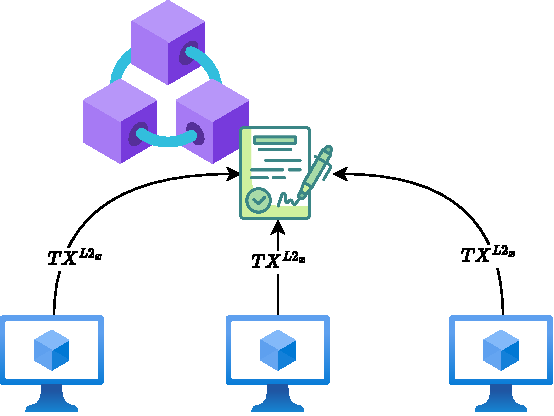
\includegraphics[width=.8\columnwidth]{\zkevmdir/figures/concepts/l2-scaling-strategies/sc-l2-tx.drawio}
\textbf{Smart Contract}
\end{column}

\end{columns}

\end{frame}




\begin{frame}{Layer 2 Design: L2 Data Availability}
\textbf{Q.} How are L2 transactions made publicly available (if so)?
\begin{itemize}
\item To achieve L2 data availability in Ethereum, currently, we can proceed in two ways:
  \begin{itemize}
  \item As a \textbf{validium} in which L2 data is managed by a group of \textbf{trusted} entities (\textbf{data managers}), being
  this approach far more \textbf{cheaper} than writing to L1.
  \item As a \textbf{rollup}, which writes L2 data in the public L1 Execution layer, meaning that the posted data will be publicly available.
  \end{itemize}
\item In the future, with the introduction of the EIP-4844, a third option opens up with \textbf{data shards}.
\end{itemize}
\end{frame}


\begin{frame}{L2 Rollups}
\begin{columns}
\begin{column}{0.65\textwidth}
\begin{figure}
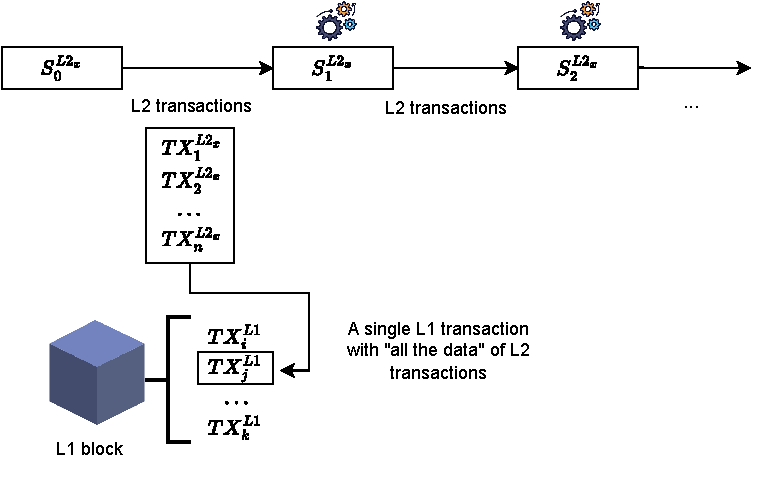
\includegraphics[width=\columnwidth]{\zkevmdir/figures/concepts/l2-scaling-strategies/l2-rollup.drawio}
\end{figure}
\end{column}

\begin{column}{0.35\textwidth}
\begin{itemize}
\item In this case, to provide data availability, we use a single L1 transaction that contains a batch of L2 transactions.
\item This idea is also called a \textbf{rollup}, because we "roll up" a bunch of L2 transactions in a single L1 transaction.
\end{itemize}
\end{column}
\end{columns}
\end{frame}

\begin{frame}{L2 Validiums}
\begin{columns}
\begin{column}{0.65\textwidth}
\begin{figure}
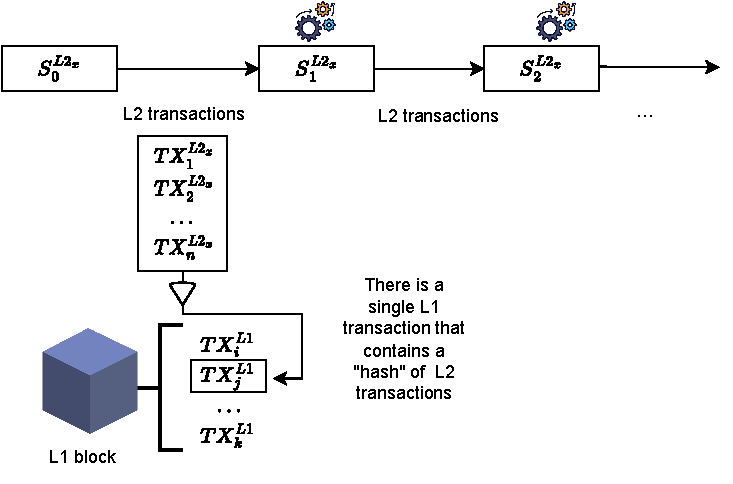
\includegraphics[width=0.9\columnwidth]{\zkevmdir/figures/concepts/l2-scaling-strategies/l2-validium.drawio}
\end{figure}
\end{column}
\begin{column}{0.35\textwidth}
  In a validium, the L1 transaction only includes a cryptographic summary of the L2 transactions.
\end{column}
\end{columns}
\end{frame}


\begin{frame}{Layer 2 Design: State Computation}
\textbf{Q.} Who processes the L2 transactions and how, and, when it is publicly considered that a new state is correctly computed?
\begin{itemize}
\item Recall that we need to compute the next L2 state $S^{L2_x}_{i+1}$ from a set of $L2^x$ transactions and the current state $S^{L2_x}_i$.
\item We can do that in several ways:
  \begin{enumerate}[a)]
  \item Centralized execution.
  \item Optimistic execution.
  \item Succinct computation verification (zk technology).
  \end{enumerate}
\end{itemize}
\end{frame}






\begin{frame}{Centralized Execution}
\begin{columns}
\begin{column}{0.6\textwidth}
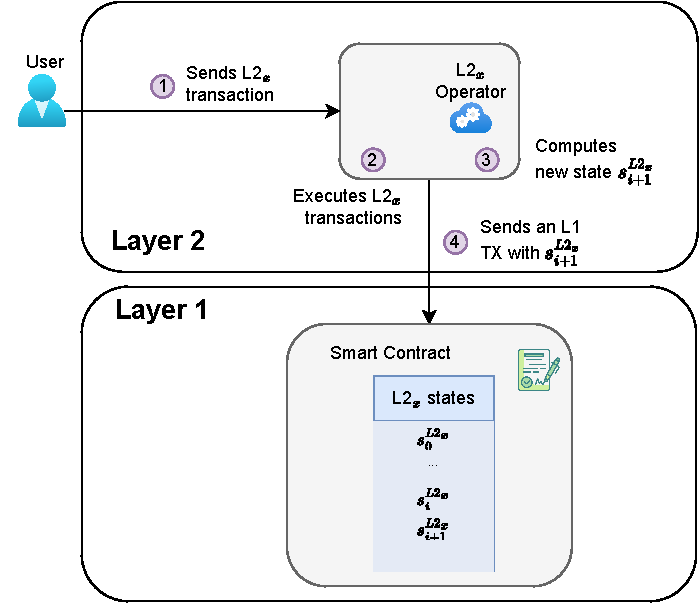
\includegraphics[width=0.9\columnwidth]{\zkevmdir/figures/concepts/l2-scaling-strategies/l2-centralized-design.drawio}
\end{column}
\begin{column}{0.4\textwidth}
\begin{itemize}
\item In this approach, the state computation is considered final quickly (takes only "seconds or minutes").
\item However, this approach has the issue of how ``we" (as external entities) dispute the L2 operator
about the correctness of an L2 state computation?
\end{itemize}
\end{column}
\end{columns}
\end{frame}





\begin{frame}{Optimistic Execution}
\begin{columns}
\begin{column}{0.45\textwidth}
\begin{itemize}
\small
\item An \textbf{Optimistic L2} provides a decentralized execution mechanism that allows
disputing the correctness of the L2 state computation.
\item With this approach, there is a (large) period of time to allow
anybody to send a \textbf{fraud proof},
proving that the state was wrongly computed (for example, a double spending transaction).
\end{itemize}
\end{column}
\begin{column}{0.53\textwidth}
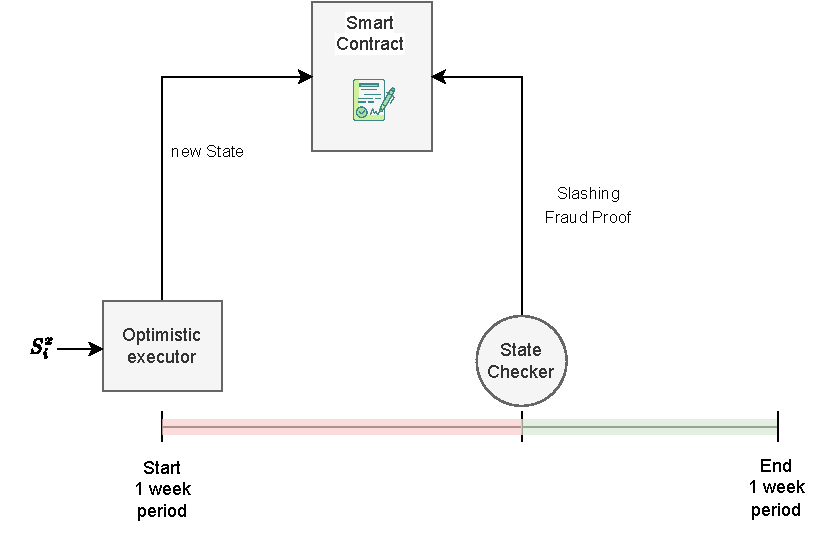
\includegraphics[width=0.93\columnwidth]{\zkevmdir/figures/concepts/l2-scaling-strategies/optimistic-fraud-proof.drawio}
\end{column}
\end{columns}
\begin{itemize}
\small
\item If the Optimistic Executor does its job correctly,
 it will earn ETH.
\item Otherwise, executor is slashed and \textbf{state checker} is rewarded 
(for providing the fraud proof).
\item Notice that the progress of the state with optimistic execution is slow,
since in general, it takes "days" to consider the state as final.
\end{itemize}
\end{frame}





\begin{frame}[t]{Succinct Execution Verification (zk* Systems)}
\begin{itemize}
\small
\item In the succinct execution verification model, instead of an optimistic executor,
we have an execution \textbf{prover}.
\item The prover can prove that an execution of a set of L2 transaction is correct.
\item The set of L2 transactions being proved is called a \textbf{batch}.
\item The prover uses \textbf{Zero-Knowledge (ZK)} technology.
\end{itemize}

\begin{columns}
\begin{column}{0.4\textwidth}
\centering
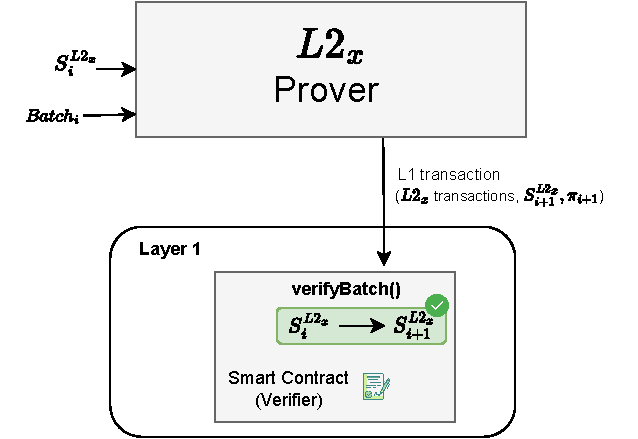
\includegraphics[width=0.9\columnwidth]{\zkevmdir/figures/concepts/l2-scaling-strategies/succinct-execution-prover-verifier.drawio}
\end{column}
\begin{column}{0.6\textwidth}
\begin{itemize}
\small
\item A smart contract in L1 is the \textbf{verifier} of the proof of the batch execution.
\item There is no possible dispute since the ZK proof proves that state is correctly computed.
\item When the smart contract executes the transaction, we say that the next state, $S^x_{i+1}$, is \textbf{consolidated}.
\item With this approach, the state computation is quickly considered final since
it takes only "seconds or minutes" to generate and validate the proof.
\end{itemize}
\end{column}
\end{columns}
\end{frame}






\begin{frame}[t]{Remarks about Prover and Verifier}
\begin{columns}
\begin{column}{0.55\textwidth}
\begin{itemize}
\item Regarding the \textbf{prover}:
  \begin{itemize}
  \item It is typically allocated in a cloud service.
  \item Uses a considerable amount of resources (mainly RAM and CPU).
  \end{itemize}

\vspace{0.2cm}
\item Regarding the \textbf{verifier}:
  \begin{itemize}
  \item The proof size is small

  (just a few bytes).
  \item The verification time is also small

  (of the order of $\mu$s).
  \item As a result, a smart contract can indeed verify proofs of L2 batch processing.
  \end{itemize}
\end{itemize}
\end{column}
\begin{column}{0.4\textwidth}
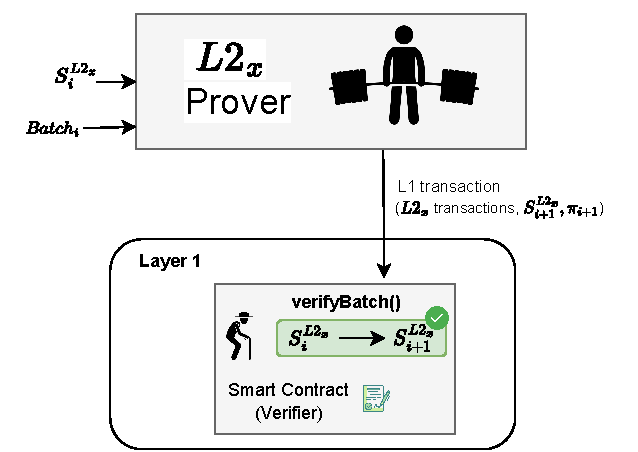
\includegraphics[width=0.95\columnwidth]{\zkevmdir/figures/concepts/l2-scaling-strategies/succinct-execution-powers.drawio}
\end{column}
\end{columns}
\end{frame}




\begin{frame}[t]{Summary of the L2 Scaling Solutions}
Scalability solutions for blockchains can be classified by two main dimensions:
  \begin{itemize}
  \item \textbf{Data availability.} Whether the data from the L2 chain is available on-chain (in L1) or off-chain (only in the L2 chain).
  \item \textbf{Mechanism to state correctness.} How the correctness of the L2 chain is guaranteed.
  \end{itemize}

\vspace{0.35cm}
\begin{figure}
\begin{tabular}{|c|c|c|}
\hline
\cellcolor{darkgray} & \cellcolor{darkgray} \color{white} Validity Proof  & \cellcolor{darkgray} \color{white} Fraud Proof \\ \hline
\cellcolor{lightgray} Data on-chain   & zkRollup       & Optimistic Rollup \\ \hline
\cellcolor{lightgray} Data off-chain  & zkValidium     & Plasma \\ \hline
\end{tabular}
\end{figure}

\centering
\vspace{0.2cm}
\url{https://l2beat.com/scaling/summary}
\end{frame}




% \begin{frame}[allowframebreaks]{Remarks about zkValidiums}
% \begin{columns}
% \begin{column}{0.35 \textwidth}
% \begin{itemize}
% \small
% \item In \textbf{zkValidium}, instead of posting all the batch data back to L1, only a cryptographic summary (a \textit{hash}) of it is posted.
% \item This means that a user cannot retrieve the L2 transactions from L1. 
% \item Instead, the user must ask a \textit{reliable} L2 operator (data manager) for these data.
% \end{itemize}
% \end{column}
% \begin{column}{0.65 \textwidth}
% \begin{figure}
% \centering
% 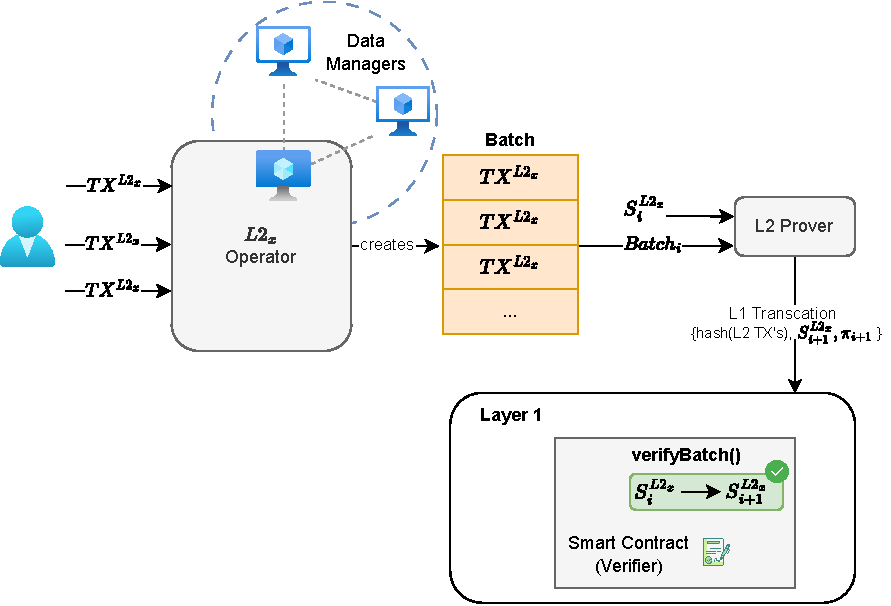
\includegraphics[width=\columnwidth]{\zkevmdir/figures/concepts/l2-scaling-strategies/validium.drawio}
% \end{figure}
% \end{column}
% \end{columns}

% \framebreak
% In case the operators do not provide the data to the user, still the ZK processing assures that the transactions included in the batch
% are always correctly processed.

% \vspace{0.2cm}
% This means that, for example: 

% \vspace{0.1cm}
%   \begin{itemize}
%   \item No one can steal your funds. 
%   \item You might see an increase in your L2 balance, but you might not know which concrete L2 transaction produced this increase.
%   \end{itemize}
% \end{frame}






\begin{frame}{L2 Applications: Simple or Rich Processing}
\begin{figure}
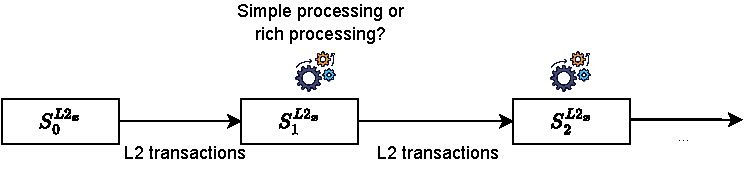
\includegraphics[width=0.6\columnwidth]{\zkevmdir/figures/concepts/l2-scaling-strategies/l2-applications.drawio}
\end{figure}

\textbf{Q.} What type of applications the L2 supports?
\begin{itemize}
\item \textbf{Simple asset transfers}, e.g. tokens or payment network with "simple processing" of the transactions.
\item \textbf{General purpose execution virtual machine}, e.g. EVM with "rich processing" of the transactions.
\end{itemize}
\end{frame}





\begin{frame}{L2 Simple Processing}
\begin{figure}
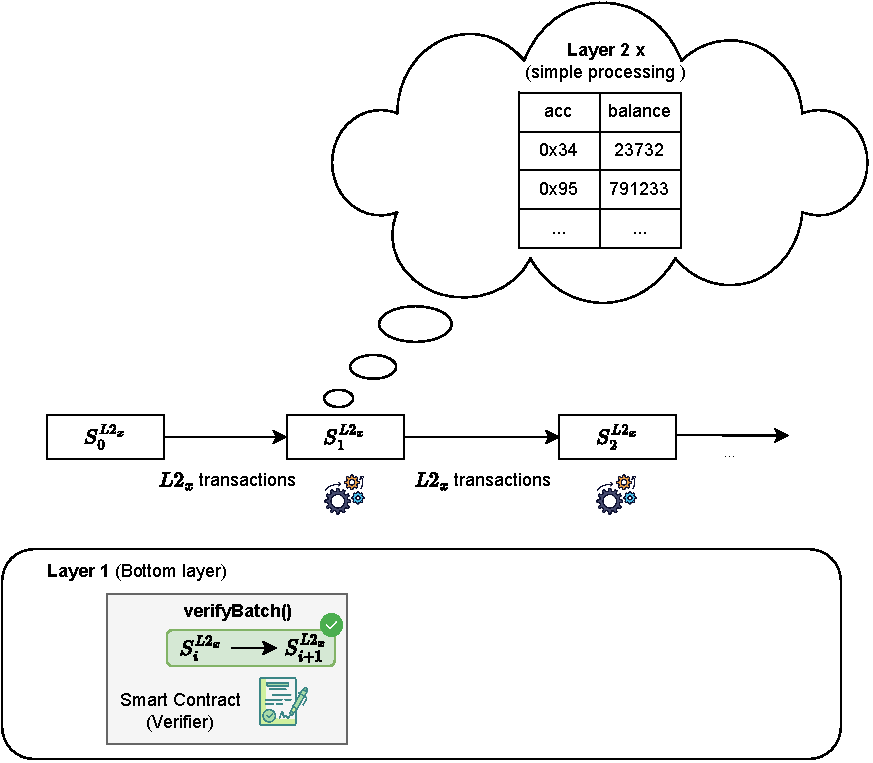
\includegraphics[width=0.53\columnwidth]{\zkevmdir/figures/concepts/l2-scaling-strategies/l2-simple-processing.drawio}
\end{figure}
\end{frame}






\begin{frame}{L2 Rich Processing (zkEVM)}
\begin{figure}
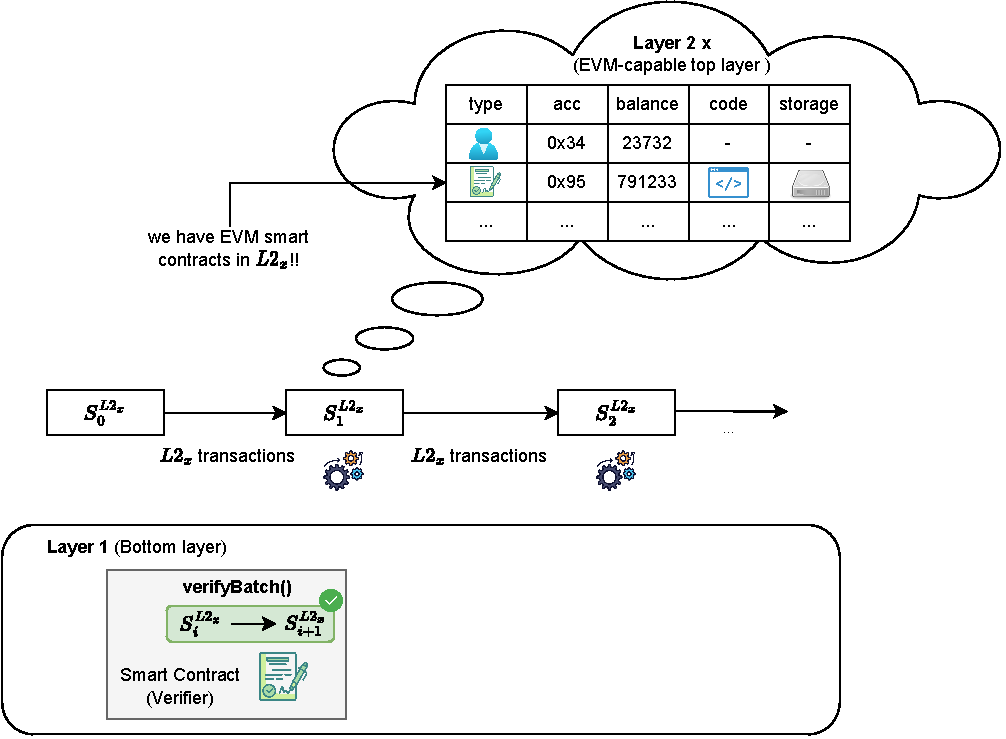
\includegraphics[width=0.6\columnwidth]{\zkevmdir/figures/concepts/l2-scaling-strategies/l2-rich-processing-zkevm.drawio}
\end{figure}
\end{frame}



\begin{frame}[fragile, allowframebreaks]{zkEVMs Compatibility/Equivalence}
\begin{figure}
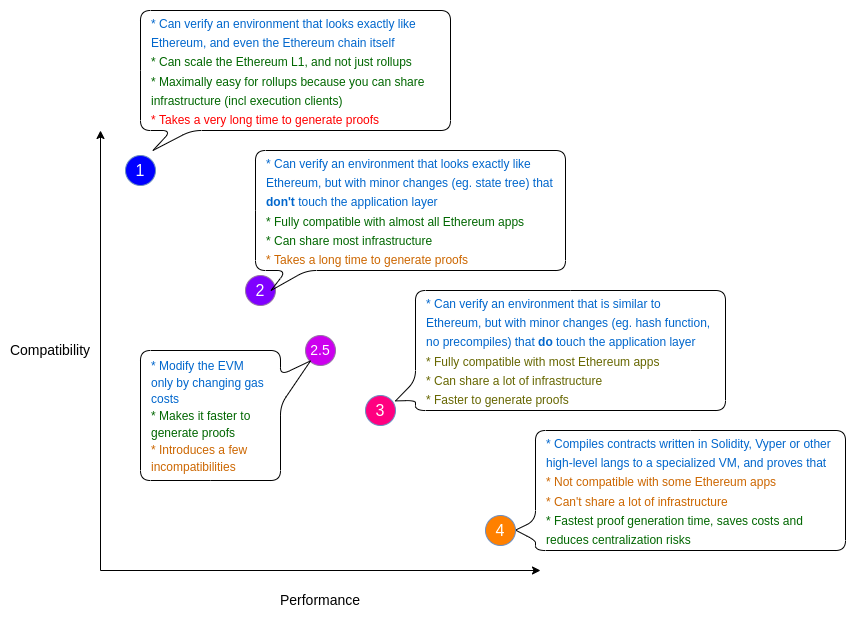
\includegraphics[width=0.6\columnwidth]{\zkevmdir/figures/architecture/intro-proving-system/zkEVM-compatibility-post-vitalik}
\end{figure}
\end{frame}




\begin{frame}{Are we Scaling with zkRollups?}
\ifPROF
\footnotesize
\textbf{++Prof:} This is a natural question since all the L2 data is somehow posted in the L1 chain.
\normalsize
\fi

\textbf{Q.} A last natural question is if we are scaling with rollups based on succinct verification.

\textbf{The answer is yes}, because the smart contract execution resources for verifying a proof are much lower
than executing individual transactions within a batch.


In fact, the majority of the cost comes from the data availability, but we can work on improve the costs of data availability.

\vspace{0.2cm}
Addressing data availability costs:
  \begin{itemize}
  \item Succinct verification of \textbf{compressed} data (for example, transaction digital signature).
  \item EIP 4844 \textbf{Proto-Danksharing}:
    \begin{itemize}
    \item Data shards are much cheaper than writing in L1 execution layer.
    \item Remark that the L1 execution layer (smart contracts) will have access to blobs in data shards.
    \end{itemize}
  \end{itemize}
\end{frame}

% !TeX document-id = {38ad272c-6b95-4178-b409-8ae7f3766667}
% !TeX spellcheck = en_US
% !TeX root = ../../build/architecture.tex
% !TeX TXS-program:compile = txs:///xelatex/[--shell-escape]


\renewcommand{\mytitle}{Polygon L2 Scaling Strategies}
\ifZEROSEC \fi
\ifSEC \section{\mytitle{}}\fi
\ifSUBSEC \subsection{\mytitle{}}\fi
\ifSUBSUBSEC \subsubsection{\mytitle{}}\fi


\begin{frame}{L2 Scaling and Strategies}
Review the road to scalability and the
L2 scaling strategies at the concepts.
\end{frame}




\begin{frame}{L2 Design for the Polygon zkEVM}
\begin{enumerate}[a)]
\item How users send L2 transactions and who receives them?
  \begin{itemize}
  \item The zkEVM uses \textbf{unicast} to let user send their transaction (calls to an RPC).
  \item The zkEVM also enables posting L2 transactions via a method in a \textbf{smart contract}
  as an anti-censorship measure (called "forced batches").
  \end{itemize}
\item How L2 transactions are made publicly available (if so)?
  \begin{itemize}
  \item The zkEVM is a \textbf{rollup}, the L2 data is available in L1.
  \end{itemize}
\item Who processes the L2 transactions and how, and, when
it is publicly considered that a new state is correctly computed?
  \begin{itemize}
  \item In the zkEVM, currently, there is a \textbf{centralized aggregator node} that proves the
 processing of the L2 transactions.
  \item However, this node cannot cheat because there is a \textbf{succinct computation verification}
  (using zero-knowledge technology).
  \end{itemize}
\item What type of applications the L2 supports? simple or rich processing?
  \begin{itemize}
  \item zkEVM is rich processing since it is an \textbf{EVM}.
  \end{itemize}
\end{enumerate}
\end{frame}
% !TeX spellcheck = en_US
% !TeX root = ../../build/architecture.tex
% !TeX TXS-program:compile = txs:///xelatex/[--shell-escape]


\renewcommand{\mytitle}{Polygon zkEVM Simplified Processing Flow}
\ifZEROSEC \fi
\ifSEC \section{\mytitle{}}\fi
\ifSUBSEC \subsection{\mytitle{}}\fi
\ifSUBSUBSEC \subsubsection{\mytitle{}}\fi


\begin{frame}{Complete Architecture of the zkEVM}
\begin{figure}
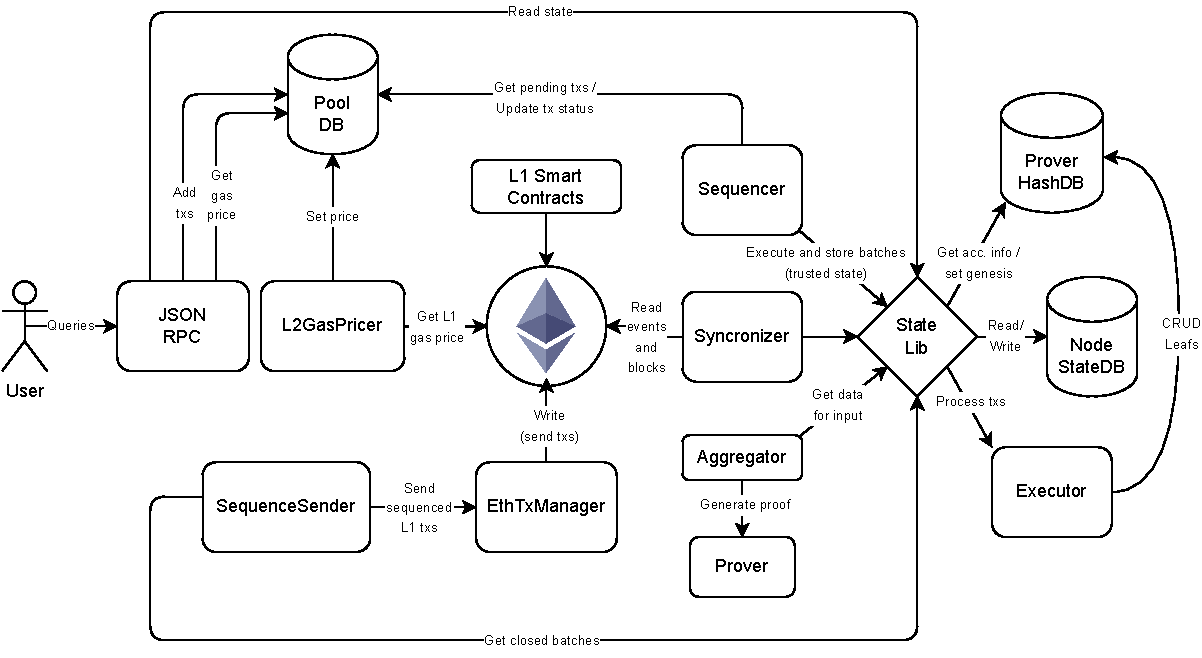
\includegraphics[width=0.8\columnwidth]{\zkevmdir/figures/architecture/zkevm-simplified-flow/architecture-map.drawio}
\end{figure}
\end{frame}




\begin{frame}[t]{Basic zkEVM L2 Processing (Simplified Flow)}
\begin{figure}
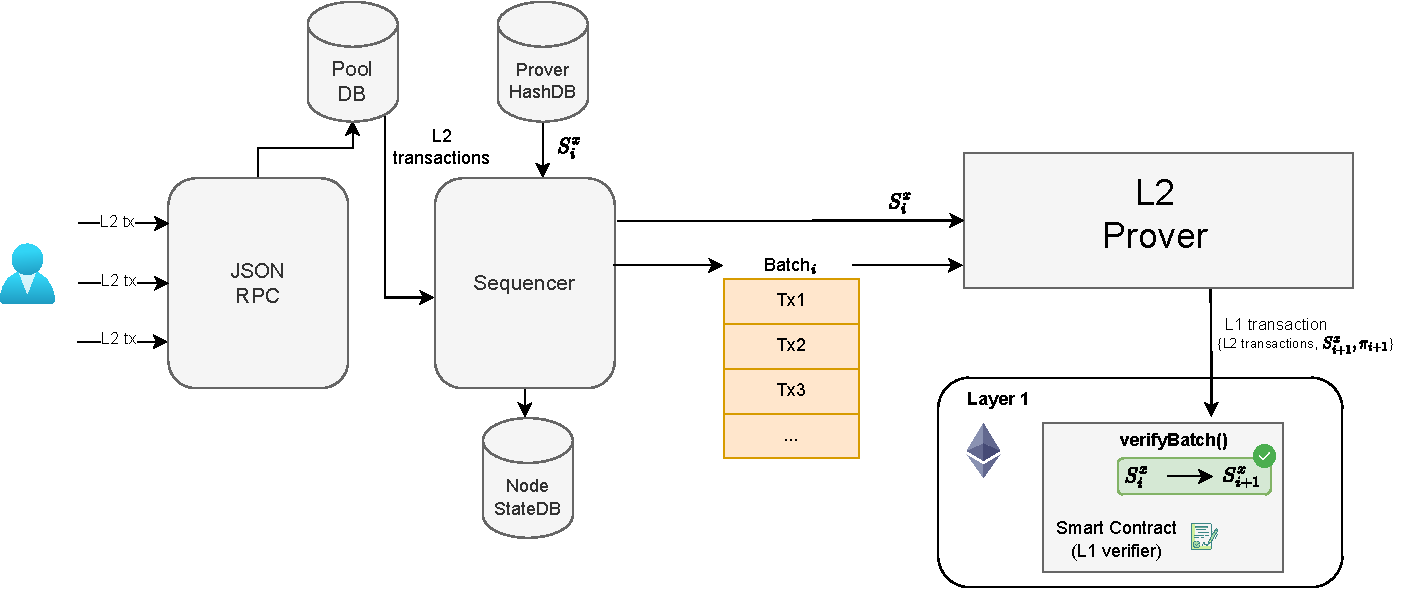
\includegraphics[width=0.95\columnwidth]{\zkevmdir/figures/architecture/zkevm-simplified-flow/zkevm-l2-processing-simplified.drawio}
\end{figure}
\end{frame}




\begin{frame}[allowframebreaks]{Processing an L2 zkEVM Transaction (Simplified Flow)}
\centering
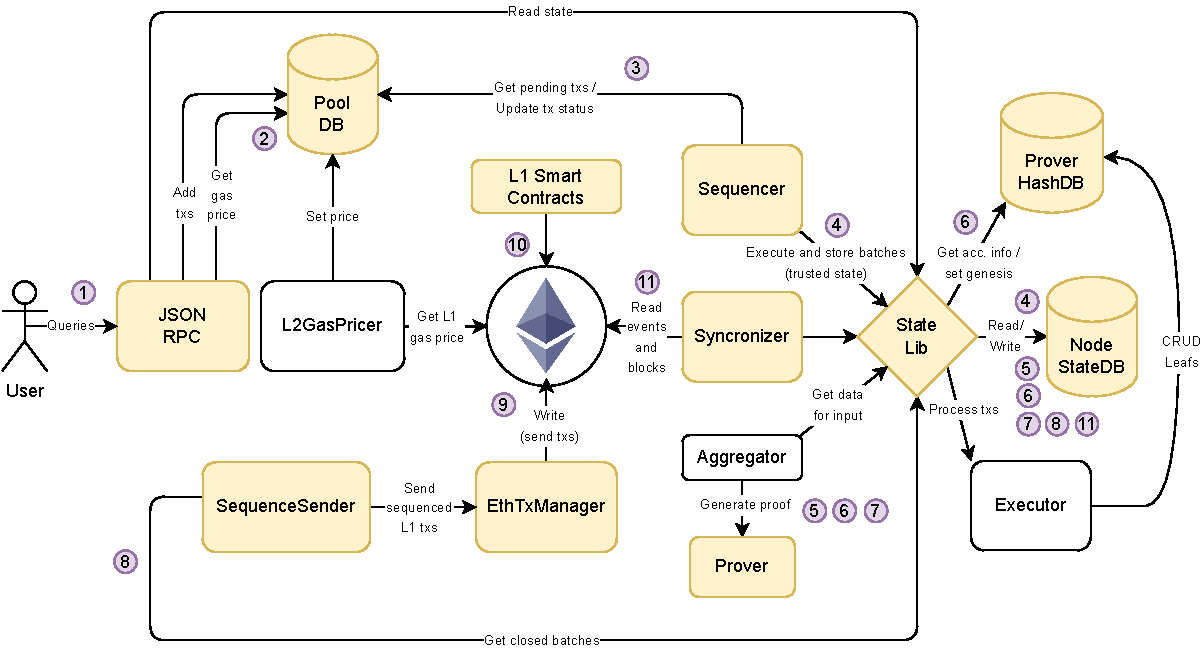
\includegraphics[width=0.8\columnwidth]{\zkevmdir/figures/architecture/zkevm-simplified-flow/architecture-map-simplified-flow.drawio}

\vspace{-0.2cm}
\tiny
\textbf{Remark.} By now, consider that white boxes don't exist. Also take into account that the functionality of some yellow boxes will be re-engineered regarding this simplified flow.

\framebreak
\begin{enumerate}
\small
\item The \textbf{user} creates a standard Ethereum transaction for the L2 (e.g. using the metamask wallet) and, 
sends it to the \textbf{JSON RPC} API of the node, which is an almost standard Ethereum JSON RPC with some extra endpoints.
\item The \textbf{JSON RPC} stores the received L2 transactions in the \textbf{pool} database of pending L2 transactions.
\item The \textbf{sequencer} creates (closes) a batch by selecting L2 transactions from the \textbf{pool} (with some criteria).
\item The \textbf{sequencer} stores the data of the new batch in the node's \textbf{StateDB}.
\item The \textbf{prover} queries the node's \textbf{StateDB} to read the data of the new batches to be proved.
\item The \textbf{prover} also reads the \textbf{HashDB} to obtain the necessary data to proof the current L2 state (root of the L2 state and hashes for Merkle proofs).
\item The \textbf{prover} generates the proof and stores it with its related data in the node's \textbf{StateDB}.

\framebreak
\item The \textbf{sequenceSender} reads the node's \textbf{StateDB} checking for any new proved batches.
\item The \textbf{sequenceSender} decides when it is the best moment to create and send the L1 transaction with the proof to the \textbf{L1 zkEVM smart contract}. The \textbf{sequenceSender} sends the transaction through the \textbf{EthTxManager}. 
The \textbf{EthTxManager} uses an L1 Ethereum node to do so (e.g. \textbf{geth/prysm}) and it makes sure that the transaction is included in a block (managing the L1 gas fees if necessary).
\item The \textbf{L1 zkEVM smart contract} processes the transaction and, if the proof is correctly verified, updates and stores the new L2 state.
\item Finally, the \textbf{synchronizer}, who is monitoring events of the \textbf{L1 zkEVM smart contract} realizes that a new batch is 
consolidated and stores this information in the node's \textbf{StateDB}.
\end{enumerate}
\end{frame}




% \begin{frame}[fragile]{Remark About Building the Software}
% \begin{itemize}
% \item Each component in a box can be instantiated in an isolated executable.
% \item The State library is imported by components (is not instantiated).
% \item While the JSON RPC is devoted to external communication, 
% the component internal communication takes place using two types of interfaces:
%   \begin{itemize}
%   \item gRPC APIs.
%   \item Postgre APIs with the databases.
%   \end{itemize}
% \item However, many components are built together into a single executable that can 
% be configured as desired when started.
% \item Finally, remark that the databases can be built as databases in a single Postgre server or
% they can be split as desired in multiple PostgreSQL servers.
% \end{itemize}
% \end{frame}

 \ARCHMAPfalse
% !TeX spellcheck = en_US
% !TeX root = ../../build/architecture.tex
% !TeX TXS-program:compile = txs:///xelatex/[--shell-escape]


\renewcommand{\mytitle}{Basic Principles of the Polygon zkEVM Proving System}
\ifZEROSEC \fi
\ifSEC \section{\mytitle{}}\fi
\ifSUBSEC \subsection{\mytitle{}}\fi
\ifSUBSUBSEC \subsubsection{\mytitle{}}\fi


\ifARCHMAP
\begin{frame}{Architecture of the zkEVM: Prover and Executor}
\begin{figure}
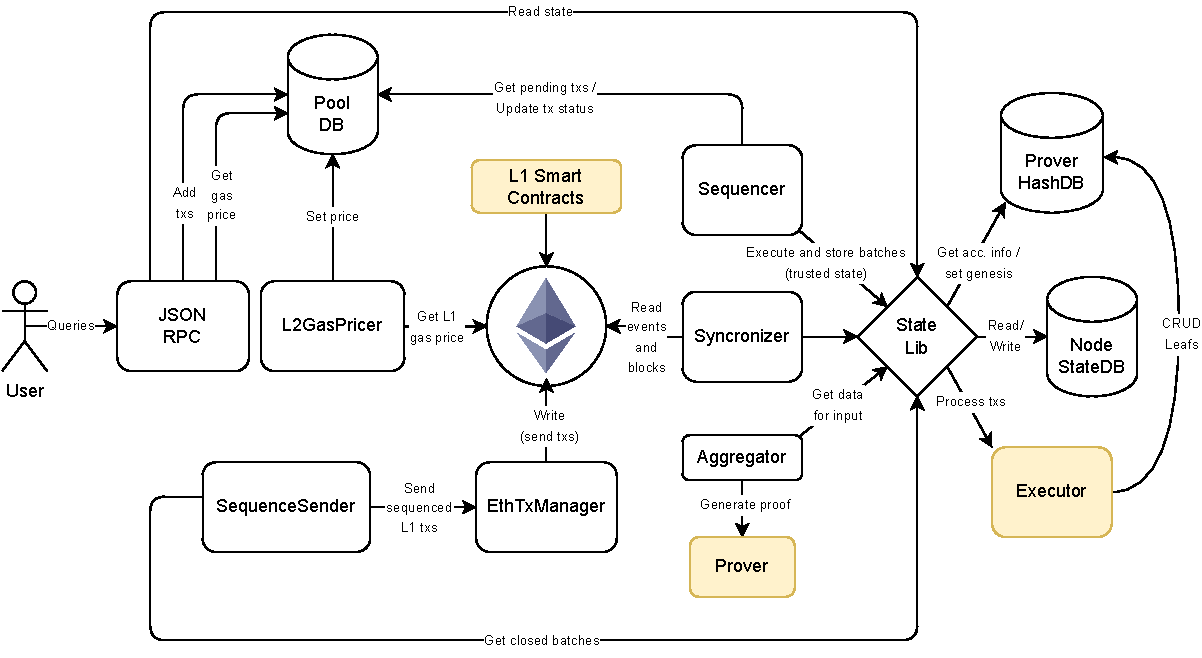
\includegraphics[width=0.85\columnwidth]{\zkevmdir/figures/architecture/intro-proving-system/architecture-map-prover-executor.drawio}
\end{figure}
\end{frame}



\begin{frame}{List of To Be Covered Concepts}
\begin{columns}
\begin{column}{0.48\textwidth}
\begin{itemize}
\item Provers. \hfill \Square
\item Execution trace. \hfill \Square
\item Witness and fixed columns. \hfill \Square
\item Executors (general purpose and computation-specific). \hfill \Square
\item zk Assembly. \hfill \Square
\item ROM of the zkEVM. \hfill \Square
\item forkId. \hfill \Square
\end{itemize}
\end{column}
\begin{column}{0.48\textwidth}
\begin{itemize}
\item PIL (Polynomial Identity Language). \hfill \Square
\item PIL2 (WIP). \hfill \Square
\item Publics and privates. \hfill \Square
\item Verifiers (Fflonk). \hfill \Square
\item Selector columns. \hfill \Square
\item zkEVM compatibility/equivalence types. \hfill \Square
\item Secondary execution matrices A.K.A state machines. \hfill \Square
\item PIL namespaces. \hfill \Square
\item State machine interconnection with lookups. \hfill \Square
\end{itemize}
\end{column}
\end{columns}
\end{frame}
\fi



\begin{frame} {Functions of the L2 Prover}
\begin{block}{Prover}
The "Prover" is a component whose main goal is to generate a \textbf{proof} that for the correct execution of a given program with an specific set of inputs. The proving process is a resource-consuming process.
\end{block}

\begin{figure}

\includegraphics[width=0.7\columnwidth]{\zkevmdir/figures/architecture/intro-proving-system/goal-prover.drawio}
\end{figure}

\begin{columns}
\begin{column}{0.7\textwidth}
\begin{itemize}
\item To generate such a proof, we first need to create an \textbf{execution trace}.
\item An execution trace is just a \textbf{matrix} (or grid) of cells with rows and columns.
\end{itemize}
\end{column}
\begin{column}{0.3\textwidth}
$$
\begin{array}{|c|c|c|c|c|}
\hline
 &  & & & \\ \hline
 &  & & &\\ \hline
 &  & & &\\ \hline
 &  & & &\\ \hline
\end{array}
$$
\end{column}
\end{columns}
\end{frame}




\begin{frame}[allowframebreaks]{Execution Trace Example}
\begin{itemize}
\item Let $x=(x_0, x_1, x_2)$ a vector of given inputs.
\item We want to implement an execution trace for the following computation:
$$[(x_0+x_1)\cdot4]\cdot x_2$$
\item Suppose that we only have the following operations available:
  \begin{enumerate}
  \item Copy inputs into cells of the execution trace.
  \item Sum two cells of the same row, and leave the result in a cell of the next row (\texttt{ADD}).
  \item Multiply by a constant, and leave the result in a cell of the next row (\texttt{TIMES4}).
  \item Multiply two cells of the same row, and leave the result in a cell of the next row (\texttt{MUL}).
  \end{enumerate}
\item Let's consider that our execution trace has $3$ columns and a bounded number of rows (so that we can fit the needed computation in it):
$$
\begin{array}{|c|c|c|}
\hline
\textbf{A} & \textbf{B} & \textbf{C} \\ \hline
a_0 & b_0 & c_0 \\ \hline
a_1 & b_1 & c_1 \\ \hline
... & ... & ...\\ \hline
a_n & b_n & c_n \\ \hline
\end{array}
$$
\item The columns of an execution trace are often called \textbf{registers} (so we may name them interchangeably).
\end{itemize}


\framebreak
\begin{itemize}
\item Suppose we are given the following inputs $x=(x_0, x_1, x_2)=(1,2,5)$.
\item We can model our desired computation $[(x_0+x_1)\cdot4]\cdot x_2$ to fit our execution trace using only the available operations as follows:
\end{itemize}

\vspace{0.3cm}
\begin{large}
\begin{table}[h!]
\centering

\begin{tabular}{|c|c|c|}
\hline
\textbf{A} & \textbf{B} & \cellcolor{lightgray} \textbf{C} \\ \hline
1 & 2 & \cellcolor{lightgray} \\ \hline
3 & & \cellcolor{lightgray} 4 \\ \hline
12 & 5 & \cellcolor{lightgray} \\ \hline
60 & & \cellcolor{lightgray} \\ \hline
\end{tabular}
\hspace{1mm}
\begin{tabular}{r}
                    \\
$[a_0=x_0, b_0=x_1]$  \\
                    \\
$[b_2 = x_2]$         \\
                    \\

\end{tabular}
\hspace{1em}
\begin{tabular}{l}
                    \\
\texttt{ADD} \\
\texttt{TIMES4} \\
\texttt{MUL} \\
\\
\end{tabular}
\end{table}
\end{large}
\end{frame}





\begin{frame}{Witness and Fixed Columns}
\begin{itemize}
\item Notice that if we change the inputs $x=(x_0, x_1, x_2)=(5,3,2)$, we can perform exactly the same computation as before but the execution trace changes (most of) its values \textbf{but not its shape}.
$$
\begin{array}{|c|c|c|}
\hline
\textbf{A} & \textbf{B} & \cellcolor{lightgray} \textbf{C} \\ \hline
5 & 3 & \cellcolor{lightgray} \\ \hline
8 & & 4 \cellcolor{lightgray} \\ \hline
32 & 2 & \cellcolor{lightgray} \\ \hline
64 & & \cellcolor{lightgray} \\ \hline
\end{array}
$$

\item The columns that depend on the input (in this case A and B) are called \textbf{witness columns}.
\item The columns that are the same for all inputs (in this case column C) are known as \textbf{fixed columns} (which we will mark in gray color).
\item Note that fixed columns don't change as they are an intrinsic part of the computation.
\end{itemize}
\end{frame}






\begin{frame}{Functions of the Executor}

\begin{block}{Executor}
The "Executor" is a component whose main purpose is to generate a (correct) execution trace from a given set of inputs.
\end{block}

\begin{figure}
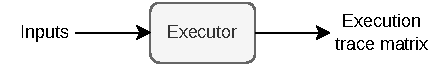
\includegraphics[width=0.65\columnwidth]{\zkevmdir/figures/architecture/intro-proving-system/general-executor}
\end{figure}
\end{frame}




\begin{frame} [allowframebreaks] {How to implement the Executor}
\textbf{Approach \#1:}
    \begin{itemize}
    \item As a component that runs just one given computation.
    \item Application Specific Integrated Circuit (ASIC) as electronic analogy: an ASIC
    is a circuit specifically designed to run, very efficiently, a single computation.
    \item We also call this executor a \textbf{native executor}.
    \end{itemize}

\begin{figure}
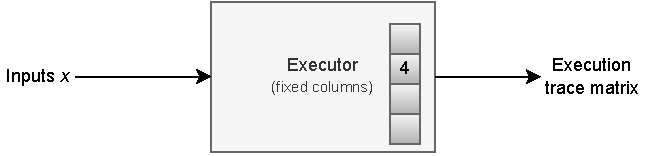
\includegraphics[width=0.9\columnwidth]{\zkevmdir/figures/architecture/intro-proving-system/executor-asic-approach.drawio}
\end{figure}


\framebreak
\textbf{Approach \#2:}
\begin{itemize}
\item As a general purpose processor, which means as a component that can run several computations or "programs".
\item In this case, the executor is as follows:
\end{itemize}
\begin{figure}[H]
\centering
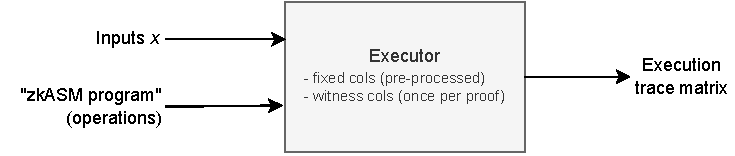
\includegraphics[width=0.9\columnwidth]{\zkevmdir/figures/architecture/intro-proving-system/executor-cpu-approach.drawio}
\end{figure}
\end{frame}





\begin{frame} {Example of an Executor that Reads Assembly Programs}
\large
Using an executor that reads assembly, we could run two zkASM programs:
\normalsize
~\\
\begin{columns}
\begin{column}{0.55\textwidth}
\textbf{Program 1: $[(x_0+x_1)\cdot4]\cdot x_2$} having $x=(x_0, x_1, x_2)=(1,2,5)$ as inputs.

\vspace{1em}

\begin{table}[h!]
\centering

\begin{tabular}{|c|c|c|}
\hline
\textbf{A} & \textbf{B} & \cellcolor{lightgray} \textbf{C} \\ \hline
1 & 2 & \cellcolor{lightgray} \\ \hline
3 & & \cellcolor{lightgray} 4 \\ \hline
12 & 5 & \cellcolor{lightgray} \\ \hline
60 & & \cellcolor{lightgray} \\ \hline
\end{tabular}
\hspace{1mm}
\begin{tabular}{r}
                    \\
$[a_0=x_0, b_0=x_1]$  \\
                    \\
$[b_2 = x_2]$         \\
                    \\

\end{tabular}
\hspace{1em}
\begin{tabular}{l}
                    \\
\texttt{ADD} \\
\texttt{TIMES4} \\
\texttt{MUL} \\
\\
\end{tabular}
\end{table}
\end{column}
\begin{column}{0.45\textwidth}
\textbf{Program 2 $(x_0\cdot16)\cdot x_1$} having $x=(x_0, x_1)=(2, 3)$ as inputs.

\vspace{1em}

\begin{table}[h!]
\centering

\begin{tabular}{|c|c|c|}
\hline
\textbf{A} & \textbf{B} & \cellcolor{lightgray} \textbf{C} \\ \hline
2 &  & \cellcolor{lightgray} 4\\ \hline
8 & & \cellcolor{lightgray} 4 \\ \hline
32 & 3 & \cellcolor{lightgray} \\ \hline
96 & & \cellcolor{lightgray} \\ \hline
\end{tabular}
\hspace{1mm}
\begin{tabular}{r}
                    \\
$[a_0=x_0]$  \\
                    \\
$[b_2 = x_1]$         \\
                    \\

\end{tabular}
\hspace{1em}
\begin{tabular}{l}
                    \\
\texttt{TIMES4} \\
\texttt{TIMES4} \\
\texttt{MUL} \\
\\
\end{tabular}
\end{table}
\end{column}
\end{columns}

\footnotesize
\url{https://github.com/0xPolygonHermez/zkevm-rom}
\normalsize
\end{frame}




%TODO WIP
\begin{frame}{Single-computation vs General-computation Executor}
\begin{figure}
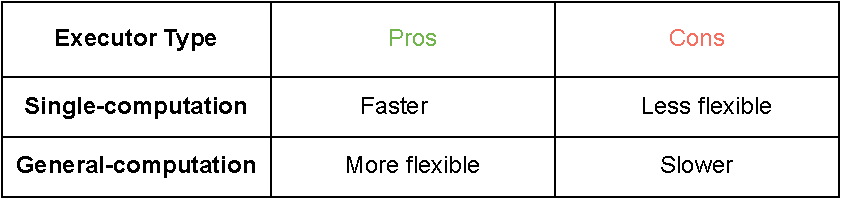
\includegraphics[scale=0.7]{\zkevmdir/figures/architecture/intro-proving-system/single-vs-general.drawio}
\end{figure}
\begin{itemize}
\small
\item The single-computation executor is faster because it does not need
to read assembly, it can implement the generation of the execution trace for the computation and
this process can be optimized for this computation.
\item However, the single-computation executor is not easy to change, test or audit.
\item In zkEVM we will have both, each one serving different purposes.
\item The single-computation executor is WIP.
\end{itemize}
\end{frame}




\begin{frame}[fragile]{zkASM: Assembly Language for the zkEVM}
\begin{itemize}

\item \textbf{zkASM} is the language developed by the team that is used to write the program that a compiler will build and the executor will interpret in order to build the execution trace.

\vspace{1em}

\begin{figure}
\begin{zkasm}
STEP => A
0                                   :ASSERT ; Ensure it is the beginning of the execution

CTX                                 :MSTORE(forkID)
CTX - %FORK_ID                      :JMPNZ(failAssert)

B                                   :MSTORE(oldStateRoot)
\end{zkasm}
\textbf{zkASM} Language Example.
\end{figure}

\vspace{1em}

\item In the repository \href{https://github.com/0xPolygonHermez/zkasmcom-vscode}{\texttt{zkasmcom-vscode}} there is a syntax highlighter for VSCode.

%npx vsce package
%code --install-extension NAME.vsix
\end{itemize}
\end{frame}






\begin{frame}{The zkASM Compiler}

\begin{block}{zkASM Compiler}
We have implemented a \href{https://github.com/0xPolygonHermez/zkasmcom}{zkASM compiler} that reads a zkASM specification file and compiles it to an output file with the list steps and instructions which the executor will consume in order to compute the execution trace.
\end{block}

\begin{figure}

\includegraphics[width=0.65\columnwidth]{\zkevmdir/figures/architecture/intro-proving-system/zkasmcom-basic.drawio}
\end{figure}

\end{frame}







\begin{frame}{ROM-based Executor}
\begin{itemize}
\item We need a \textbf{general-computation} executor because:
  \begin{itemize}
  \item Our implementation of the EVM evolves.
  \item The EVM itself also evolves.
  \end{itemize}

\item An architecture with assembly programs is faster to develop, test and audit than a specific implementation.

\item We call the Ethereum program that processes EVM transactions the \textbf{EVM ROM} (Read Only Memory) or simply the \textbf{ROM}.
\end{itemize}
\end{frame}




\begin{frame}{\texttt{forkId}}
\begin{itemize}
\item By changing the ROM, we make our L2 zkEVM more and more closer to the L1 EVM.
\item So we have versions of the zkEVM ROM.
\item Each of these versions will be denoted with an identifier called
\texttt{forkId}.
\item Another advantage of using a ROM-based approach is that we can test small parts of the assembly program
in isolation.
\item Finally, mention that:
  \begin{itemize}
  \item We are also developing a native executor (we will see why later).
  \item Having the two approaches allows us to check that execution traces generated match.
  \end{itemize}
\end{itemize}
\end{frame}




\ifARCHMAP
\begin{frame}{List of To Be Covered Concepts}
\begin{columns}
\begin{column}{0.48\textwidth}
\begin{itemize}
\item Provers. \hfill \CheckedBox
\item Execution trace. \hfill \CheckedBox
\item Witness and fixed columns. \hfill \CheckedBox
\item Executors (general purpose and computation-specific). \hfill \CheckedBox
\item zk Assembly. \hfill \CheckedBox
\item ROM of the zkEVM. \hfill \CheckedBox
\item forkId. \hfill \CheckedBox
\end{itemize}
\end{column}
\begin{column}{0.48\textwidth}
\begin{itemize}
\item PIL (Polynomial Identity Language). \hfill \Square
\item PIL2 (WIP). \hfill \Square
\item Publics and privates. \hfill \Square
\item Verifiers (Fflonk). \hfill \Square
\item Selector columns. \hfill \Square
\item zkEVM compatibility/equivalence types. \hfill \Square
\item Secondary execution matrices A.K.A state machines. \hfill \Square
\item PIL namespaces. \hfill \Square
\item State machine interconnection with lookups. \hfill \Square
\end{itemize}
\end{column}
\end{columns}
\end{frame}
\fi



\begin{frame}{Execution Correctness}
The execution correctness is enforced by a set of constraints that must be fulfilled by the execution trace:

\vspace{1em}
\begin{columns}[t]
\begin{column}{0.2\columnwidth}
\centering
\textbf{Program (computation): $(x_0+x_1)\cdot 4]\cdot x_2$} \\
\vspace{1em}
\begin{tabular}{|c|c|c|}
\hline
\textbf{A} & \textbf{B} & \cellcolor{lightgray} \textbf{C} \\ \hline
1 & 2 & \cellcolor{lightgray} \\ \hline
3 & & \cellcolor{lightgray} 4 \\ \hline
12 & 5 & \cellcolor{lightgray} \\ \hline
60 & & \cellcolor{lightgray} \\ \hline
\end{tabular}
\end{column}

\begin{column}{0.5 \columnwidth}
\centering
\vspace{-.5em}
\textbf{Constraints:}
\begin{align*}
&a_0 = x_0 \\
&b_0 = x_1 \\
&a_1 = a_0 + b_0 \\
&a_2 = a_1 \cdot 4 \\
&b_2 = x_2 \\
&a_3 = a_2 \cdot b_2
\end{align*}
\end{column}
\end{columns}
\end{frame}





\begin{frame}{The PIL Language and its Compiler}
\begin{itemize}
\item In our cryptographic backend:
  \begin{itemize}
  \item Each column is transformed into a polynomial (of the degree the number of rows).
  \item Constraints are defined over these polynomials.
  \item We describe constraints using a language called \textbf{PIL (Polynomial Identity Language)}.
  \end{itemize}
\end{itemize}

\small
\begin{block}{PIL Compiler}
We have implemented a \href{https://github.com/0xPolygonHermez/pilcom}{PIL compiler} that reads a PIL specification file and compiles it to an output file with the list of constraints and a format that can be consumed by the prover.
\end{block}
\begin{figure}

\includegraphics[width=0.65\columnwidth]{\zkevmdir/figures/architecture/intro-proving-system/pilcom-basic.drawio}
\end{figure}
\begin{itemize}
\item The repository \href{https://github.com/0xPolygonHermez/pilcom-vscode}{\texttt{pilcom-vscode}} contains a PIL syntax highlighter for VSCode.
\end{itemize}
\ifPROF
\footnotesize
\textbf{++Prof:} Latter we will see some PIL, but comment that a PIL specification can have a loop and the compiler
outputs the list of constraints which is what the prover in fact needs.
\normalsize
\fi
\end{frame}






\begin{frame}[allowframebreaks]{Publics and Privates}
\begin{itemize}
\item With zk-technology, we can create execution traces
where some of the inputs are \textbf{private}.
\vspace{0.3cm}
\begin{columns}
\begin{column}{0.33\textwidth}
\textbf{Example 1} \centering
$$
\begin{array}{|c|c|c|}
\hline
\textbf{A} & \textbf{B} & \cellcolor{lightgray} \textbf{C} \\ \hline
1 \cellcolor{green} & 2 \cellcolor{green}
& \cellcolor{lightgray} \\ \hline
3 & & 4 \cellcolor{lightgray} \\ \hline
12 & 5 \cellcolor{green} &
\cellcolor{lightgray} \\ \hline
60 \cellcolor{green} & & \cellcolor{lightgray}
\\ \hline
\end{array}$$
\end{column}
\begin{column}{0.33\textwidth}
\textbf{Example 2} \centering
$$
\begin{array}{|c|c|c|}
\hline
\textbf{A} & \textbf{B} & \cellcolor{lightgray} \textbf{C} \\ \hline
1 \cellcolor{green} & 2 \cellcolor{orange} &
\cellcolor{lightgray} \\ \hline
3 & & 4 \cellcolor{lightgray} \\ \hline
12 & 5 \cellcolor{green} &
\cellcolor{lightgray} \\ \hline
60 \cellcolor{green} & &
\cellcolor{lightgray} \\ \hline
\end{array}$$
\end{column}
\begin{column}{0.33\textwidth}
$\begin{array}{|c|}
\hline
\cellcolor{green}\\ \hline
\end{array}$
: publics \\ \vspace{0.2cm}
$\begin{array}{|c|} \hline
\cellcolor{orange}\\ \hline
\end{array}$
: privates \\ \vspace{0.2cm}
$\begin{array}{|c|} \hline
\cellcolor{lightgray}\\ \hline
\end{array}$
: fixed
\end{column}
\end{columns}
\vspace{0.3cm}
\item Recall that columns A and B are \textbf{witness} while the C column is
\textbf{fixed}.
\end{itemize}


\framebreak
\begin{columns}
\begin{column}{0.48\textwidth}
$$
\begin{array}{|c|c|c|}
\hline
\textbf{A} & \textbf{B} & \cellcolor{lightgray} \textbf{C} \\ \hline
1 \cellcolor{green} & 2 \cellcolor{orange} &
\cellcolor{lightgray} \\ \hline
3 & & 4 \cellcolor{lightgray} \\ \hline
12 & 5 \cellcolor{green} &
\cellcolor{lightgray} \\ \hline
60 \cellcolor{green} & &
\cellcolor{lightgray} \\ \hline
\end{array}$$
\end{column}
\begin{column}{0.48\textwidth}
\begin{itemize}
\item \textbf{Public inputs}: \{1, 5\}
\item \textbf{Private inputs}: \{2\}
\item \textbf{Output (public)}: \{60\}
\item \textbf{Publics}: \{{1, 5, 60}\}
\end{itemize}
\end{column}
\end{columns}

\vspace{0.5cm}
In this execution trace design, input $x_1$ is
private, while inputs $x_0$ and $x_2$ are public and
the output is also public.

\vspace{0.1cm}
Publics are enforced by constraints.
\end{frame}




\begin{frame}{Generating and Verifying Proofs}
\begin{figure}[H]
\centering
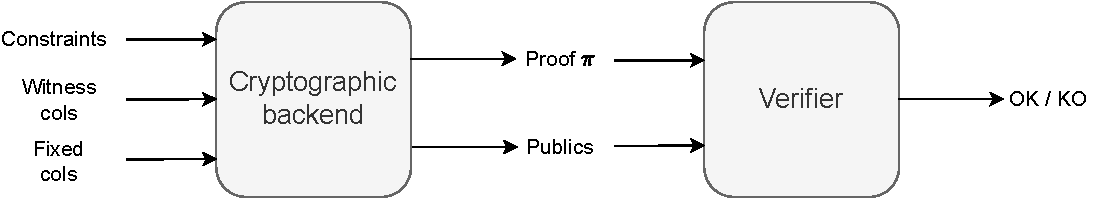
\includegraphics[scale=0.65]{\zkevmdir/figures/architecture/intro-proving-system/generating-verifying-proofs.drawio}
\end{figure}
\begin{itemize}
\small
\item With a valid proof $\pi$, the verifier is convinced that
the execution of the computation in question is correct for the given public inputs.

\item $\pi$ is small and needs a small amount of
resources to be validated.
\item In our case, currently we use a backend cryptographic system whose final verifier is \textbf{FFlonk}.
\item \textbf{Note}: A smart contract in the L1 execution layer can verify the proof implementing a FFlonk verifier (and therefore validate the computation of a new state from a batch) with $\approx 200K$ gas.
\end{itemize}
\end{frame}



\begin{frame}[fragile]{Example of Usage of a Private Input}

A typical example of using a private input is to prove the knowledge of
the pre-image of a hash without revealing this pre-image value:

\begin{figure}
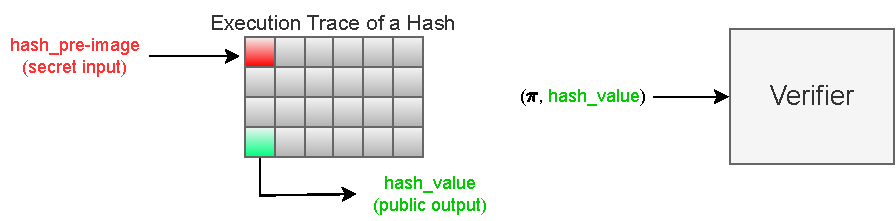
\includegraphics[width=0.9\columnwidth]{\zkevmdir/figures/architecture/intro-proving-system/private-input-hash-example.drawio}
\end{figure}

\ifPROF
\vspace{0.2cm}
\scriptsize
\textbf{++Prof:} We can show some variants with a concatenation of another public input value.
\normalsize
\fi

\end{frame}







\begin{frame}{Shaping Execution Traces}
\begin{itemize}
\item In an execution trace, each row is in charge of validating an \textbf{zkASM operation} or \textbf{part of an operation}.
\item For example, suppose that we are given a set of $3$ operations \texttt{OP1, OP2} and \texttt{OP3}.
\item These operations change the next\footnote{Primes mean next value of some column, e.g. $a'$ means the next value in the \textbf{A} column.}
value of the \textbf{A} column.
\begin{align*}
&\texttt{OP1}: a'=a+b+c \\
&\texttt{OP2}: a'=a+b+c+d+e\\
&\texttt{OP3}: a'=a+b+c+d+e+f+g+h
\end{align*}
\item Consider also that we have an execution trace matrix of $6$ columns.

\vspace{0.1cm}
\begin{columns}
\begin{column}{0.4 \textwidth}

\scriptsize

\begin{table}[h!]
\begin{tabular}{|c|c|c|c|c|c|}
\hline
\textbf{A} & \textbf{B} & \textbf{C} & \textbf{D} & \textbf{E} & \textbf{F} \\ \hline
 &  &  & & &\\ \hline
 &  &  &  &  &  \\ \hline
 &  &  &  &  & \\ \hline
 &  &  &&& \\ \hline
\end{tabular}
\end{table}
\end{column}
\begin{column}{0.36 \textwidth}
\item \textbf{Q.} Can we fit this computation inside the matrix? how?
\end{column}
\end{columns}
\vspace*{5mm}
\end{itemize}
\end{frame}





\begin{frame}{Shaping Execution Traces: Strategies}
\begin{itemize}
\item We can adopt two straightforward strategies:
  \begin{enumerate}[a)]
  \item Increasing the number of columns so that we can fit every summand.
  \item Use the next row in order to fit some of the remaining summands of the operation.
  \end{enumerate}

\vspace{1em}

\item Using the second approach, we can define an execution matrix in which \texttt{OP3}
uses two rows:
\begin{align*}
&\texttt{OP1}: a'=a+b+c \\
&\texttt{OP2}: a'=a+b+c+d+e\\
&\texttt{OP3}: a'=a+b+c+d+e+f+b'+c'
\end{align*}

\scriptsize
\vspace{1em}

\begin{table}[h!]
\begin{tabular}{|c|c|c|c|c|c|}
\hline
\textbf{A} & \textbf{B} & \textbf{C} & \textbf{D} & \textbf{E} & \textbf{F} \\ \hline
$a_0$ & $b_0$ & $c_0$ & & &\\ \hline
$a_1$ & $b_1$ & $c_1$ & $d_1$ & $e_1$ & \\ \hline
\cellcolor{yellow} $a_2$ & \cellcolor{yellow} $b_2$ & \cellcolor{yellow}  $c_2$ & \cellcolor{yellow} $d_2$ & \cellcolor{yellow} $e_2$ & \cellcolor{yellow} $f_2$ \\ \hline
\cellcolor{green} $a_3$ & \cellcolor{yellow}  $b_3$ & \cellcolor{yellow}  $c_3$ &&& \\ \hline
\end{tabular}
\hspace{1em}
\begin{tabular}{c}
              \\
$\mathtt{OP1}$ \\
$\mathtt{OP2}$ \\
$\mathtt{OP3}$ \\
$             $ \\
\end{tabular}
\end{table}
\end{itemize}
\end{frame}






\begin{frame}[allowframebreaks]{Execution Trace Design Strategies}
Number of rows and columns?

\vspace{0.25cm}
\begin{itemize}
\item The maximum number of rows might be fixed by a cryptographic back-end
(this is the case of our current back-end).
\item The fewer rows used, the faster the prover is.
\item In practice, $\# rows=2^n$ for some natural $n \in \mathbb{N}$.
\item More or less columns?  Adding columns also increases proving time.
\end{itemize}


\framebreak
\begin{columns}
\begin{column}{0.48\textwidth}
\begin{table}[h!]
\begin{tabular}{c}
$             $ \\
$\mathtt{OP1}$ \\
$\mathtt{OP2}$ \\
$             $
\end{tabular}
\begin{tabular}{|c|c|c|c|c|c|}\hline
$\mathbf{A}$ & $\mathtt{B}$ & $\mathtt{C}$ & $\mathtt{D}$ & $\mathtt{E}$ & $\mathtt{F}$ \\ \hline
$a_0$ & $b_0$ & $c_0$ & \cellcolor{cyan} & \cellcolor{cyan} & \cellcolor{cyan} \\ \hline
$a_1$ & $b_1$ & $c_1$ & $d_1$ & $e_1$ & \cellcolor{cyan} \\ \hline
\cellcolor{green} $a_2$ & \cellcolor{cyan} & \cellcolor{cyan} & \cellcolor{cyan} & \cellcolor{cyan} & \cellcolor{cyan} \\ \hline
\end{tabular}
\end{table}
\vspace{0.3cm}
\end{column}
\begin{column}{0.48\textwidth}
\texttt{OP1}: $a'=a+b+c$
\\ \texttt{OP2}: $a'=a+b+c+d+e$
\\ \textit{$6$ columns and $3$ rows.}
\\ \textit{$18$ cells but $9$ of them unused.}
\end{column}
\end{columns}
\begin{columns}
\begin{column}{0.48\textwidth}

\vspace{0.2cm}
\begin{table}[h!]
\begin{tabular}{c}
$             $ \\
$\mathtt{OP1}$ \\
$\mathtt{OP2}$ \\
$             $
\end{tabular}
\begin{tabular}{|c|c|c|}\hline
$\mathbf{A}$ & $\mathtt{B}$ & $\mathtt{C}$ \\ \hline
$a_0$ & $b_0$ & $c_0$ \\ \hline
$a_1$ & $b_1$ & $c_1$ \\ \hline
$a_2$ & $b_2$ & \cellcolor{green}$c_2$ \\ \hline
\end{tabular}
\end{table}
\end{column}
\begin{column}{0.48\textwidth}
\texttt{OP1}: $a'=a+b+c$
\\ \texttt{OP2}: $c'=a+b+c+a'+b'$
\\ \textit{$3$ columns and $3$ rows.}
\\ \textit{$9$ cells and all of them used. }
\end{column}
\end{columns}
\#unused\_cells depends on the instructions executed and the execution matrix shape.
\end{frame}





\begin{frame}{Selector Columns}
\begin{columns}
\begin{column}{0.48\textwidth}
\begin{table}[h!]
\begin{tabular}{c}
$             $ \\
$\mathtt{OP1}$ \\
$\mathtt{OP2}$ \\
$             $
\end{tabular}
\begin{tabular}{|c|c|c|}\hline
$\mathbf{A}$ & $\mathtt{B}$ & $\mathtt{C}$ \\ \hline
$a_0$ & $b_0$ & $c_0$ \\ \hline
$a_1$ & $b_1$ & $c_1$ \\ \hline
$a_2$ & $b_2$ & $c_2$ \\ \hline
\end{tabular}
\end{table}
\end{column}
\begin{column}{0.48\textwidth}
\texttt{OP1}: $a+b+c-a'=0$
\\ \texttt{OP2}: $a+b+c+a'+b'-c'=0$
\end{column}
\end{columns}


\begin{itemize}
\small
\item Since we are using constraints with columns (not cells), we need to add \textbf{selector columns}.
\item Selector columns are used to control wether the constraints apply or not (meaning whether we are performing this or that operation).
\end{itemize}

\begin{columns}
\begin{column}{0.48\textwidth}
\begin{table}[h!]
\begin{tabular}{c}
$             $ \\
$\mathtt{OP1}$ \\
$\mathtt{OP2}$ \\
$             $
\end{tabular}
\begin{tabular}{|c|c|c|c|c|}\hline
$\mathbf{A}$ & $\mathtt{B}$ & $\mathtt{C}$ & $\mathtt{OP1}$ & $\mathtt{OP2}$ \\ \hline
$a_0$ & $b_0$ & $c_0$ & 1 & 0 \\ \hline
$a_1$ & $b_1$ & $c_1$ & 0 & 1\\ \hline
$a_2$ & $b_2$ & $c_2$ & & \\ \hline
\end{tabular}
\end{table}
\end{column}
\begin{column}{0.48\textwidth}
\begin{align*}
op1*(1-op2)*(a+b+c-a') &+  \\
op2*(1-op1)*(a+b+c+a'+b'-c') &= 0
\end{align*}
\end{column}
\end{columns}
\end{frame}





\begin{frame}{The Execution Trace and the zkEVM}
\begin{itemize}
\small
\item In our current cryptographic backend, we have a shape that is pre-fixed for the execution trace.
\item Also, we don't know exactly what EVM opcodes (and as a consequence zkEVM operations) will be executed, 
since this depends on the particular transactions of the L2 batch.
\item The pre-fixed shape fixes in turn the amount of computation that we can do, which
in our case is the amount and type of L2 transactions for which we can generate a proof.
\item  In general, it is hard to optimize the shape of a single execution trace matrix:
\end{itemize}
\begin{columns}
\begin{column}{0.36\textwidth}
\begin{enumerate}
\footnotesize
\item \textbf{Narrow matrices may easily hit the max row limit}, which is about $2^{23}$
(fixed by the cryptographic back-end).
\item \textbf{Wide matrices might be inefficient} for mixing many different instructions.
\end{enumerate}
\end{column}
\begin{column}{0.55\textwidth}
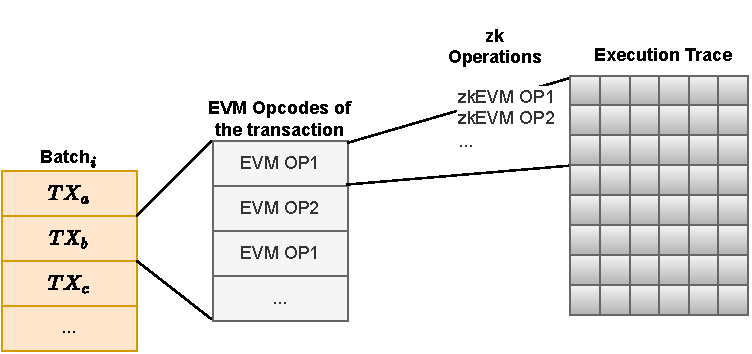
\includegraphics[width=\columnwidth]{\zkevmdir/figures/architecture/intro-proving-system/batch-evmopcode-zkop-trace.drawio}
\end{column}
\end{columns}
\end{frame}




\begin{frame}[fragile, allowframebreaks]{zkEVMs Compatibility/Equivalence}
\begin{columns}
\begin{column}{0.46\textwidth}
\begin{itemize}
\footnotesize
\item A layer 2 is EVM compatible or equivalent if it can run EVM byte code without modifying the underlying smart contract logic. 
\item EVM compatibility allow L2's to use existing Ethereum smart contracts, patterns, standards, and tooling.
\item Being EVM compatible is important for the widespread adoption of these L2 since this allows using existing tools can be used.
\item In practice, there are several types of compatibility.
\item \textbf{Type 1:} Fully Ethereum equivalent, i.e. they do not change any part of the Ethereum system but generating proofs
can take several hours.
\end{itemize}
\end{column}
\begin{column}{0.51\textwidth}
\begin{itemize}
\footnotesize
\item \textbf{Type 2:} Fully EVM-equivalent, but changes some different internal representations like how they store the state of the chain, for the purpose of improving ZK proof generation times.
\item \textbf{Type 2.5:} Fully EVM-equivalent, except they use different gas costs for some operations to "significantly improve worst-case prover times".
\item \textbf{Type 3:} Almost EVM-equivalent zkEVMs make sacrifices in exact equivalence to further enhance prover times and simplify EVM development.
\item \textbf{Type 4:} High-level language equivalent zkEVMs compile smart contract source code written in a high-level language to a friendly language for zk, resulting in faster prover times but potentially introducing incompatibilities and limitations.
\end{itemize}
\end{column}
\end{columns}




\framebreak
\begin{figure}
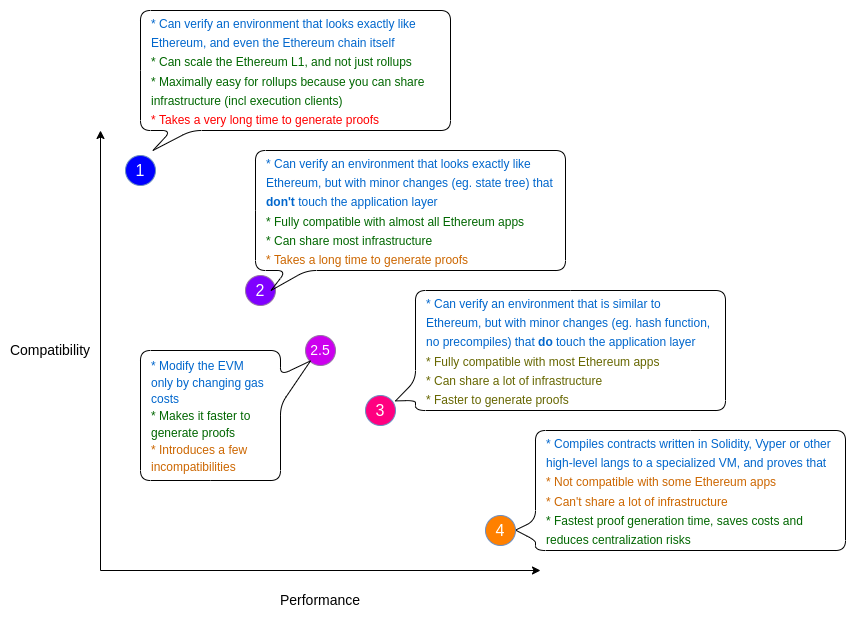
\includegraphics[width=0.6\columnwidth]{\zkevmdir/figures/architecture/intro-proving-system/zkEVM-compatibility-post-vitalik}
\footnotesize
\url{https://vitalik.ca/general/2022/08/04/zkevm.html}
\end{figure}
\end{frame}






\begin{frame}{Motivational Example: Implementing an EXP Operation}
\begin{itemize}
\small
\item Let's assume that our cryptographic backend only allows to define constraints with additions and multiplications.
\item Let's consider also that we want to implement a exponentiation operation (\texttt{EXP}).
\item Then, we can use several rows doing multiplications to implement \texttt{EXP}.
\item A portion of the execution trace (that implements $2^5 = 32$) could be:
\begin{columns}
\begin{column}{0.2\textwidth}
$$
\begin{array}{|c|c|c|}
\hline
\textbf{A} & \textbf{B} & \textbf{C} \\ \hline
2 & 5 & 2  \\ \hline
2 & 4 & 4  \\ \hline
2 & 3 & 8  \\ \hline
2 & 2 & 16 \\ \hline
2 & 1 & 32 \\ \hline
\end{array}$$
\end{column}

\begin{column}{0.7\textwidth}
\small
An incomplete (\textbf{uncorrected}) set of constraints:

\vspace{0.1cm}
\begin{enumerate}
\small
\item $a'=a$ \quad 
(the \textbf{A} column represents the base)
\item $b'=b-1$ \quad 
(the \textbf{B} column stores the decreasing exponent)
\item $c'=c\cdot a$ \quad 
(the \textbf{C} column stores the intermediate results)
\end{enumerate}
\end{column}
\end{columns}

\vspace{0.2cm}
\item If we want to implement this operation in the main Execution Trace, note that
we are going to spend several rows per \texttt{EXP} operation.
\item In fact, a variable number of rows per \texttt{EXP} operation depending on the exponent.
\end{itemize}
\end{frame}










\begin{frame} {Secondary Execution Trace Matrices and Lookup Arguments}
\begin{itemize}
\item The previous approach leads to a very complicated set of constraints together with a huge amount
of consumed rows by operations, which is quite an unwanted scenario.
\item Another approach is to use \textbf{tailor-made secondary execution traces for specific operation(s)}:
  \begin{itemize}
  \item In this approach, there is a \textbf{main execution trace} and there are also \textbf{secondary execution traces}.
  \item In the cryptographic back-end, we use a mechanism called \textbf{lookup argument} to \textbf{link} these execution trace matrices.
  \item In particular, the lookup argument provides the constraints necessary to check that certain cells of a row in an execution trace matrix match other cells in a row of another execution trace matrix.
  \end{itemize}
\item So, another approach for our \texttt{EXP} operation is to implement it in a secondary execution trace matrix
and link the main execution trace with the secondary trace with a \textbf{lookup argument}.
\end{itemize}
\end{frame}





\begin{frame}{Main Trace with Delegated Operation checks}
\begin{columns}
\begin{column}{0.3\textwidth}
$$\begin{array}{|c|c|c|c|}
\hline
\textbf{A} &  \textbf{B} & \textbf{C} &  \textbf{EXP}\\ \hline
\cdots & \cdots & \cdots & 0 \\ \hline
2 & 5 & 32 & 1 \\ \hline
\cdots & \cdots & \cdots & 0 \\ \hline
\cdots & \cdots & \cdots & 0 \\ \hline
\cdots & \cdots & \cdots & 0 \\ \hline
\cdots & \cdots & \cdots & 0 \\ \hline
3 & 2 & 9 & 1 \\ \hline
\cdots & \cdots & \cdots & 0 \\ \hline
\cdots & \cdots & \cdots & 0 \\ \hline
& & & \\ \hline
\end{array} $$
\end{column}
\begin{column}{0.7\textwidth}
\begin{itemize}
\item In the main execution trace, each \texttt{EXP} operation occupies
just one row.
\item Notice that we introduced the \textbf{EXP} selector to indicate
when the \texttt{EXP} operation is being performed.
\item For the first \texttt{EXP} operation, inputs are 2
and 5 and the result is 32.
\item The correctness of the result will be
validated in a secondary execution matrix.
\end{itemize}
\end{column}
\end{columns}
\end{frame}




\begin{frame}{State Machine (SM) Concept and Lookup Between SMs}
\begin{columns}
\begin{column}{0.35\textwidth}
\begin{itemize}
\item An execution trace matrix can be seen as a
set of states (\textbf{state machine}), in which
each row is a state.
\item We will use both, the terms "execution trace matrix" and "state machine" interchangeably.
\end{itemize}
\end{column}
\begin{column}{0.3\textwidth}
\textbf{Main state machine} \centering

\vspace{-0.7cm}
$$ \begin{array}{|c|c|c|c|}
\hline
\textbf{A} &  \textbf{B} & \textbf{C} &  \textbf{EXP}\\
\hline
\cdots & \cdots & \cdots & 0 \\ \hline
2  \cellcolor{yellow} & 5 \cellcolor{yellow} &
32 \cellcolor{yellow} & 1 \cellcolor{yellow} \\
\hline
\cdots & \cdots & \cdots & \cdots \\ \hline
3  \cellcolor{yellow} & 2 \cellcolor{yellow} & 9
\cellcolor{yellow} & 1 \cellcolor{yellow} \\ \hline
\cdots & \cdots & \cdots & 0 \\ \hline
\end{array} $$
\begin{flushleft} \hspace{0.6cm}
$ \begin{array}{|c|}
  \hline \cellcolor{yellow} \\ \hline
\end{array}$
: Lookup
\end{flushleft}
\end{column}
\begin{column}{0.3\textwidth}
\textbf{EXP state machine} \centering

\vspace{-0.7cm}
$$\begin{array}{|c|c|c|c|c|}
\hline
\textbf{A} & \textbf{B} & \textbf{C} & \textbf{D}
& \textbf{EXP} \\ \hline
2 & 5 & 2 & 5 & 0 \\ \hline
2 & 5 & 4 & 4 & 0 \\ \hline
2 & 5 & 8 & 3 & 0 \\ \hline
2 & 5 & 16 & 2 & 0 \\ \hline
2 \cellcolor{yellow} & 5 \cellcolor{yellow} &
32 \cellcolor{yellow} & 1 & 1
\cellcolor{yellow}\\ \hline
3 & 2 & 3 & 2 & 0 \\ \hline
3 \cellcolor{yellow} & 2 \cellcolor{yellow} & 9
\cellcolor{yellow} & 1 & 1 \cellcolor{yellow} \\ \hline
& & & & \\ \hline
\end{array} $$
\end{column}
\end{columns}

\vspace{0.2cm}
\begin{itemize}
\item Constraints in the secondary SM enforce the
correctness of the \texttt{EXP} operation.
\item In the main SM, we just put the inputs/outputs,
that we call \textit{"free"}, in a single row.
\end{itemize}
\end{frame}








\ifPILFOURBYTEEXAMPLE
\begin{frame}[fragile]{Example: Byte4 SM}
\begin{columns}
\begin{column}{0.5\textwidth}
\[
\begin{array}{|a|c|c|c|}
\hline
\textbf{SET} &  \textbf{free} & \textbf{out} &  \textbf{out'}\\ \hline
0 & $\textsf{0xba04}$ & \cellcolor{black} \color{white} \mathbf{0x00000000} & $\textsf{0x0000ba04}$ \\ \hline
1 & $\textsf{0x3ff2}$ & \cellcolor{black} \color{white} \mathbf{0x0000ba04} & $\textsf{0xba043ff2}$ \\ \hline
0 & $\textsf{0x4443}$ & \cellcolor{black} \color{white} \mathbf{0xba043ff2} & $\textsf{0x00004443}$ \\ \hline
1 & $\textsf{0xc1d1}$ & \cellcolor{black} \color{white} \mathbf{0x00004443} & $\textsf{0x4443c1d1}$ \\ \hline
0 & $\textsf{0xd11e}$ & \cellcolor{black} \color{white} \mathbf{0x4443c1d1} & $\textsf{0x0000d11e}$ \\ \hline
1 & $\textsf{0x6ab9}$ & \cellcolor{black} \color{white} \mathbf{0x0000d11e} & $\textsf{0xd11e6ab9}$ \\ \hline
0 & \cdots          & \cellcolor{black} \color{white} \mathbf{0xd11e6ab9} & \cdots   \\ \hline
\cdots & \cdots & \cdots & \cdots    \\ \hline
\end{array}
\]
\end{column}
\begin{column}{0.5\textwidth}
\begin{itemize}
\item In one row (also named clock), the first 16-bit free input is moved to $\textsf{out}$.
\item In the following clock, the next 16-bit free input is moved+concatenated to $\textsf{out}$. 
\item We introduce the \texttt{SET} constant polynomial to manage the alternating move and move+concatenation.
\item Note that we have valid 32-bit numbers in the \texttt{out} column.
\end{itemize}
\end{column}
\end{columns}
\end{frame}








\begin{frame}[fragile]{Example: PIL for the Byte4 SM}
\begin{columns}
\begin{column}{0.5\textwidth}
\begin{itemize}
\item The computation is enforced with the following constraint:
\[
\textsf{out}' = (1 - \textsf{SET}) \cdot \textsf{free} + \textsf{SET} \cdot (2^{16} \cdot \textsf{out} + \textsf{free}).
\]
\end{itemize}
\begin{pil}
namespace Global(%N);
    pol constant L1;
    pol constant BYTE2; // [0,1,...,65535]

namespace Byte4(%N);
  pol constant SET; // [0, 1, 0, 1, 0, 1, ...]
  pol commit free;
  pol commit out;

  // Identities 
  free in Global.BYTE2; // Lookup: input in [0,...,65535]
  out' = (1 - SET)*free + SET*(2**16*out + free);
\end{pil}
\end{column}
\begin{column}{0.5\textwidth}
\begin{itemize}
\item Notice that when $\textsf{SET} = 0$, then $\textsf{out}' = \textsf{free}$, i.e., $\textsf{out}$ is set to be the first input. 
\item In contrast, when $\textsf{SET} = 1$, then $\textsf{out}' = 2^{16} \cdot \textsf{out} + \textsf{free}$, i.e., the previous input (stored in $\textsf{out}$) is set to be the upper part of $\textsf{out}$, while the second input is set to be the lower part of $\textsf{out}$. 
\item To achieve soundness, we must also check that both free inputs are numbers of $2$ bytes.
\end{itemize}
\end{column}
\end{columns}

\ifPROF
\vspace{0.2cm}
\scriptsize
\textbf{++Prof:}
\$ node ../../pilcom/src/pil.js example.pil -o output.pil.json
\normalsize
\fi
\end{frame}
\fi




\begin{frame}{The PIL of the zkEVM}
\begin{itemize}
\item Recall that there is a \href{https://github.com/0xPolygonHermez/pilcom}{PIL compiler} that reads a PIL specification file and compiles it to an output file with the list of constraints and a format that can be consumed by the prover.
\item In the PIL language, the state machines (subexecution matrices) are called \texttt{namespaces}.
\item In the \href{https://github.com/0xPolygonHermez/zkevm-proverjs}{zkevm-proverjs} repository, you can find the \href{https://github.com/0xPolygonHermez/zkevm-proverjs/tree/main/pil}{PIL specification of the zkEVM} under the pil directory.
\end{itemize}

\ifPROF
\vspace{0.2cm}
\footnotesize
\textbf{++Prof:} 

- In the PIL compiler README explain namespaces and trace size.

- Show PIL of the zkEVM: lookups, publics and some constraints.
\fi
\end{frame}




\begin{frame}{Remarks about the Computation and the Shape of SMs}
\begin{columns}
\begin{column}{0.48 \textwidth}
\begin{itemize}
\small
\item The columns of each state machine are defined by
the design of its corresponding execution trace.
\item Due to limitations of our current cryptographic backend, all the SM must have the same number of rows.
\item The computation of an L2 batch can have branches and loops and hence, 
each L2 batch execution can use a different number of operations in the zkEVM.
\item As a result, the number of rows used at each SM depends on the
number of operations of each type during the batch execution.
\end{itemize}
\end{column}

\begin{column}{0.5 \textwidth}
\begin{itemize}
\small
\item Since the number of rows is fixed (and the same for all State Machines) we
can have \textit{unused} rows.
\item But, what is more important is that obviously, \textbf{the size of the computation being proved must fit 
in the execution trace matrices available}.
\end{itemize}
\begin{figure}
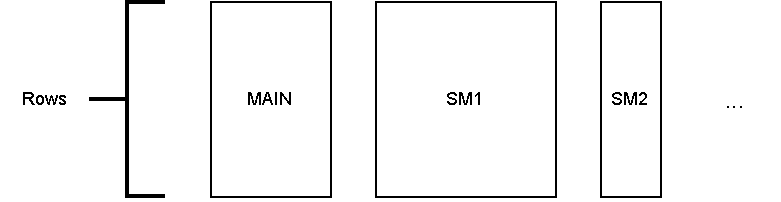
\includegraphics[width=\columnwidth]{\zkevmdir/figures/architecture/intro-proving-system/shape-state-machines.pdf}
\end{figure}

\ifPROF
\vspace{0.2cm}
\scriptsize
\textbf{++Prof:} Draw in the picture when we have unused rows and a possible overflow.
\normalsize
\fi

\end{column}
\end{columns}
\end{frame}



%TODO WIP
\begin{frame}{PIL Evolution: PIL2 (WIP)}
\begin{itemize}
\item Currently, we are under the development of a new version of PIL called \textbf{PIL2}.

\vspace{0.2cm}
\item PIL2 is designed to operate with a more powerful cryptographic backend that is able to 
generate as many subexecution traces as required by the batch processing so that we never run out of rows.

\vspace{0.2cm}
\item We are also agreeing with the rest of the "zk projects" at Polygon a format for the PIL output file called "pilout".
\end{itemize}
\end{frame}





\begin{frame} {Recap of the Prover}
\begin{figure}
\centering
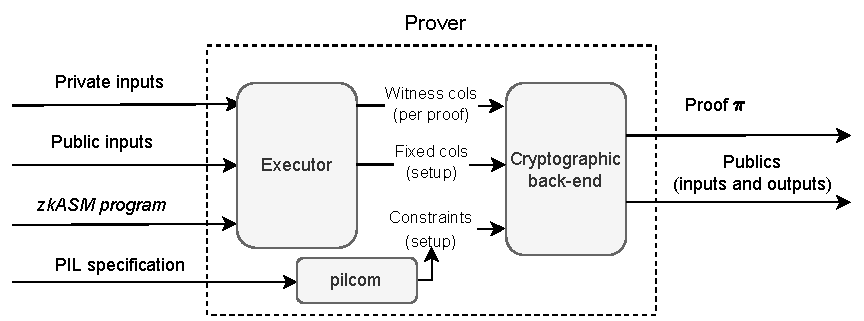
\includegraphics[width=0.95\columnwidth]{\zkevmdir/figures/architecture/intro-proving-system/prover-diagram.drawio}
\end{figure}

\footnotesize
\textbf{Note.} The files containing the pre-processed fixed columns and the processed witness columns for the zkEVM are temporary stored in binary files and are quite large (>100Gb).
\end{frame}



\begin{frame}{Recap of the Verifier}
\begin{itemize}
\item In our previous example:

\vspace{1em}

\begin{columns}
\begin{column}{0.40\textwidth}
$$
\begin{array}{|c|c|c|} \hline
\textbf{A} & \textbf{B} & \cellcolor{lightgray} \textbf{C} \\ \hline
1 \cellcolor{green} & 2 \cellcolor{orange} & \cellcolor{lightgray} \\ \hline
3 & & 4 \cellcolor{lightgray} \\ \hline
12 & 5 \cellcolor{green} & \cellcolor{lightgray} \\ \hline
60 \cellcolor{green} & & \cellcolor{lightgray} \\ \hline
\end{array}
$$
\end{column}

\begin{column}{0.26\textwidth}
$ \begin{array}{|c|} \hline \cellcolor{green}\\ \hline \end{array} $
: publics \\ \vspace{0.2cm}
$ \begin{array}{|c|} \hline \cellcolor{orange}\\ \hline \end{array} $
: privates \\ \vspace{0.2cm}
$ \begin{array}{|c|} \hline \cellcolor{lightgray}\\ \hline\end{array}$
: fixed
\end{column}
\begin{column}{0.33\textwidth}
\begin{itemize}
\item \textbf{Public inputs}: \{1, 5\}
\item \textbf{Private inputs}: \{2\}
\item \textbf{Output} (public): \{60\}
\item \textbf{Publics}: \{{1, 5, 60}\}
\end{itemize}
\end{column}
\end{columns}
\vspace{0.3cm}
\item Then the verifier:
\end{itemize}
\begin{figure}[H]
\centering
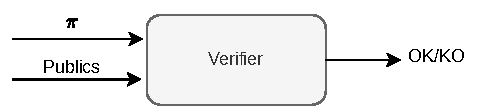
\includegraphics[width=0.6\columnwidth]{\zkevmdir/figures/architecture/intro-proving-system/verifier-diagram}
\end{figure}
\end{frame}






\ifARCHMAP
\begin{frame}{List of Covered Concepts}
\begin{columns}
\begin{column}{0.48\textwidth}
\begin{itemize}
\item Provers. \hfill \CheckedBox
\item Execution trace. \hfill \CheckedBox
\item Witness and fixed columns. \hfill \CheckedBox
\item Executors (general purpose and computation-specific). \hfill \CheckedBox
\item zk Assembly. \hfill \CheckedBox
\item ROM of the zkEVM. \hfill \CheckedBox
\item forkId. \hfill \CheckedBox
\item PIL (Polynomial Identity Language). \hfill \CheckedBox
\end{itemize}
\end{column}
\begin{column}{0.48\textwidth}
\begin{itemize}
\item PIL2 (WIP). \hfill \CheckedBox
\item Publics and privates. \hfill \CheckedBox
\item Verifiers (Fflonk). \hfill \CheckedBox
\item Selector columns. \hfill \CheckedBox
\item zkEVM compatibility/equivalence types. \hfill \CheckedBox
\item Secondary execution matrices A.K.A state machines. \hfill \CheckedBox
\item PIL namespaces. \hfill \CheckedBox
\item State machine interconnection with lookups. \hfill \CheckedBox
\end{itemize}
\end{column}
\end{columns}
\end{frame}
\fi


\end{document}


